       \documentclass[12pt,pdftex,letterpaper]{article}
            \usepackage{setspace}
            \usepackage[dvips,]{graphicx} %draft option suppresses graphics dvi display
%            \usepackage{lscape}
%            \usepackage{latexsym}
%            \usepackage{endnotes}
%            \usepackage{epsfig}
%           \singlespace
            \setlength{\textwidth}{6.5in}
            \setlength{\textheight}{9in}
            \addtolength{\topmargin}{-\topmargin} 
            \setlength{\oddsidemargin}{0in}
            \setlength{\evensidemargin}{0in}
            \addtolength{\headsep}{-\headsep}
            \addtolength{\topskip}{-\topskip}
            \addtolength{\headheight}{-\headheight}
            \setcounter{secnumdepth}{2}
%            \renewcommand{\thesection}{\arabic{section}}
            % \renewcommand{\footnote}{\endnote}
            \newtheorem{proposition}{Proposition}
            \newtheorem{definition}{Definition}
            \newtheorem{lemma}{lemma}
            \newtheorem{corollary}{Corollary}
            \newtheorem{assumption}{Assumption}
            \newcommand{\Prob}{\operatorname{Prob}}
            \clubpenalty 5000
            \widowpenalty 5000
            \renewcommand{\baselinestretch}{1.35}
            
            \usepackage{amsmath}
            \usepackage{amsthm}
            \usepackage{amsfonts}
            \usepackage{amssymb}
            \usepackage{bbm}
            \usepackage{float}
            \usepackage{graphicx}
            \usepackage{multirow}
            \usepackage{natbib}
            \usepackage{longtable}
            \usepackage{subcaption}
            \usepackage{enumerate}
            \usepackage{setspace}
            \usepackage{cancel}
            \usepackage{hyperref}
            \usepackage{xr}
%            \usepackage[nofiglist, notablist, nomarkers]{endfloat}
            
            \newcommand{\der}[2]{\frac{\text{d}#1}{\text{d}#2}}
            \newcommand{\pd}[2]{\frac{\partial#1}{\partial#2}}
            \newcommand{\E}{\operatorname{E}}
            \newcommand{\N}{\mathbb{N}}
            \newcommand{\R}{\mathbb{R}}
            
            \newcommand{\Health}{h}
            \newcommand{\ExpHealth}{\overline{\Health}}
            \newcommand{\TopHealth}{H}
            \newcommand{\Report}{x}
            \newcommand{\Age}{j}
            \newcommand{\Sex}{s}
            \newcommand{\AgeMin}{\underline{\Age}}
            \newcommand{\AgeMax}{\overline{\Age}}
            \newcommand{\AgeIncr}{\hat{\Age}}
            \newcommand{\Corr}{\rho}
            \newcommand{\HealthInitMean}{\mu_0}
            \newcommand{\HealthInitStd}{\sigma_0}
            \newcommand{\Cut}{\chi}
            \newcommand{\DiscreteCut}{\zeta}
            \newcommand{\MortParam}{\theta}
            \newcommand{\CorrParam}{\gamma}
            \newcommand{\HealthParam}{\beta}
            \newcommand{\LatentParam}{\alpha}
            \newcommand{\HealthShock}{\epsilon}
            \newcommand{\ShockMean}{\mu}
            \newcommand{\ShockStd}{\sigma}
            \newcommand{\MixProb}{q}
            \newcommand{\ReportShock}{\eta}
            \newcommand{\TypeProb}{p}
            \newcommand{\TypeProbPcvd}{\widetilde{\TypeProb}}
            \newcommand{\ReportStd}{\varsigma}
            \newcommand{\Data}{X}
            \newcommand{\ParamVec}{\Delta}
            \newcommand{\LivPrb}{\Omega}
            \newcommand{\CumLivPrb}{\omega}
            \newcommand{\TransPrb}{\Xi}
            \newcommand{\HealthDstn}{\Lambda}
            \newcommand{\ReportPrb}{\Psi}
            \newcommand{\HealthDstnPcvd}{\widetilde{\Lambda}}
            \newcommand{\LL}{\pi}
            \newcommand{\RootDir}{..}
            \newcommand{\FigsDir}{\RootDir/Figures}
            \newcommand{\TablesDir}{\RootDir/Tables}
						
\begin{document}


\title{Self-Reported Health Status \\ and Latent Health Dynamics}
\author{Matthew N. White$^\dagger$}
\date{\today}

\begin{singlespace}
\maketitle

\begin{abstract}
	Most dynamic structural models that include health as a state variable use categorical self-reported health status (SRHS) as their sole empirical measure of health. Almost universally, transition probabilities among discrete health states are calculated directly from one-wave-ahead transitions observed in panel data, either as simple fractions of respondents or by reduced form methods.  The predicted dynamics of SRHS generated from these calculations rapidly deviate from empirical transitions more than one wave ahead, as the assumption of a Markov(1) process is not satisfied.  Consequently, these models are not well calibrated to accurately match the long term dynamics of individual health, and quantitative predictions that rely on agents making decisions based on such dynamics might be unreliable.  As an alternative, this paper specifies a model in which SRHS is a noisy measure of a continuous latent health state. I estimate the model by maximum likelihood on several panel datasets, exploiting long sequences of SRHS rather than simple wave-to-wave transitions.  I demonstrate that the latent health model is able to match both short-run and long-run SRHS transitions up to twenty years in the future; it also fits other features of empirical SRHS dynamics, including apparent duration dependence. Moreover, the measure of latent health inferred from observations of SRHS is at least as good at predicting other outcomes (including mortality, labor supply, and medical expenses) as SRHS itself.
\end{abstract}

\end{singlespace}

\noindent \textbf{JEL Classification:} I19, C33

\vspace{0.25cm}

\noindent \textbf{Keywords:} \textit{latent health, panel data, maximum likelihood estimation}

\vspace{0.5cm}
\begin{singlespace}
	\noindent \textbf{Notes:} Many thanks to Svetlana Pashchenko, Chung Tran, and Fabian Lange for helpful conversations early in this project's life-cycle.  A complete reproduction archive is available at \href{http://www.github.com/mnwhite/HiddenHealth-public}{\texttt{http://www.github.com/mnwhite/HiddenHealth-public}}, including all data and code used in the project, as well as many auxiliary figures not included in the main text.
	
	\vspace{0.5cm}
	
	\noindent \textbf{Conflicts of Interest:} I affirm that I have no conflicts of interest for this project.
	
	\vspace{1cm}
	
	\small
	\noindent $\dagger$ Univ of Delaware, Dept of Economics (416B Purnell Hall, Newark DE 19716);  mnwecon@udel.edu
\end{singlespace}


\thispagestyle{empty}

\newpage


\newlength{\TableWidth}

\section{Introduction}\label{sec:Intro}

Dynamic structural models of individuals often concern decisions for which health status is an important state variable.  For example, \cite{DeNardi10} examine how the strong serial correlation of medical expenses motivates the saving behavior of the elderly, and \cite{Aizawa19} models how workers sort between jobs depending on whether they offer employer-sponsored insurance.  Papers in this vein predominantly model health as a discrete state and use categorical \textit{self-reported health status} (SRHS) as their sole empirical measure of health.\footnote{A typical SRHS survey question asks the respondent, ``Would you say your health in general is excellent, very good, good, fair, or poor?'' as in the Panel Study of Income Dynamics.}  Despite its simplicity, SRHS has been shown to be a good predictor of mortality and medical expenses (\cite{Idler97}) as well as labor supply decisions (\cite{Bound91}), and is strongly correlated with both clinical measures of health (\cite{LaRue79}) and itemized self-reports of more specific aspects of health (\cite{Blundell17}).

In this paper, I argue that while SRHS is an acceptable measure of health status for structural models, the literature has erred in its treatment of the dynamics of SRHS.  Almost universally, modelers assume that the discrete health state follows a Markov(1) process, with the distribution of subsequent states determined only by current SRHS (and demographic variables). They estimate this process using one-wave-ahead transitions of SRHS from panel data, either by simple frequency counts or reduced form methods. This approach treats SRHS literally, taking it as an accurate representation of ``true health''.  However, it is easy to show that SRHS is not Markov(1) in the data, and that the predicted distribution of health states generated by such ``simple dynamics'' swiftly deviates from the empirical distribution more than one wave ahead.  To the extent that model agents' optimal behavior depends on their beliefs about their future health prospects (e.g.\ through the need to maintain a buffer of assets against catastrophic health expenses), counterfactual simulation of these models is unreliable if the long run dynamics of individual health are incorrectly specified.

Rather than treating SRHS as an accurate measure of true health, I provide strong evidence that SRHS is better interpreted as a noisy signal of a continuous latent health state.  In this context, a change in an individual's self-report of categorical health from one wave of a survey to the next might reflect mere transitory reporting error (e.g.\ the respondent's mood), not a change in his true latent health.  I show that when a fairly parsimonious model of the data-generating process for SRHS is estimated by maximum likelihood, it is able to reproduce conditional distributions of SRHS up to twenty years ahead while still matching short run, one-wave transitions.  Health is much more persistent in the estimated latent health model than in the usual approach that does not account for reporting error in SRHS.

The estimation method exploits long sequences of SRHS observations for each respondent, rather than just one-wave-ahead transitions. The goal of the estimation is to separate transitory reporting shocks from the underlying dynamics of latent health while accounting for the econometrician's uncertainty about a respondent's latent health by tracking its nonparametric distribution.  In Section \ref{sec:Results}, I present estimation results for a dataset that combines two long panel surveys, the Panel Study of Income Dynamics and the Health and Retirement Study, but similar results are achieved from each dataset independently, or when estimated on short panel data from the Medical Expenditure Panel Study.


\subsection{Health Dynamics in Structural Models}\label{sec:StructuralSRHS}

Almost universally in the dynamic structural literature, representations of individual health have at most one continuous dimension;\footnote{The one exception known to me is \cite{Ozkan17}, who models physical and preventive health capital stocks, but these objects do not have analogues in the data from which to estimate a dynamic process.} more typically, health is represented as a discrete (often binary) state, usually taken directly from SRHS data. The question eliciting SRHS is straightforward and general, leading to very low rates of refusal or other non-response.  Most commonly, the top three categories (excellent, very good, and good) are combined into a ``healthy'' state and the bottom two categories (fair and poor) into an ``unhealthy'' state.

Across papers, the probability of transitioning between the two health states is calculated by simple fractions of the data (usually conditional on age, sex, education, and other observables) or estimated in reduced form as a logit or probit on observable characteristics. Whether two or five discrete states are used, the health state is universally assumed to follow a Markov(1) process. The health process is usually calibrated outside of the main estimation by reduced form methods, with little or no justification of the Markov(1) assumption.\footnote{See the Online Appendix for a more complete discussion of how each paper discussed below specifies and estimates health dynamics.}

This practice dates to at least \cite{RustPhelan97}, who model the health state of a living individual as binary, with bad health indicated by answering affirmatively to either of two questions about disability and daily activity. Likewise, \cite{LowPistaferri15} model transitions among three levels of work limitations (none, moderate, and severe), using data from the Panel Study of Income Dynamics. Both papers estimate the dynamics of disability level directly from one-wave-ahead transitions in panel data.

Both \cite{BlauGilleskie06} and \cite{BlauGilleskie08} specify the health state as binary and based on SRHS, estimating its dynamics using data from the Health and Retirement Study. \cite{Khwaja10} presents another dynamic discrete choice model estimated by maximum likelihood on HRS data, estimating transitions among the five SRHS categories as a multinomial logit. In each paper, SRHS is treated as a representation of true health, and there is no reference to the model's ability to fit transitions more than one wave ahead.

Three papers by a well known research team all employ the same approach to modeling health dynamics. Contemporaneous work in \cite{French11} and \cite{DeNardi10} estimate one-wave-ahead transition probabilities between binary health states based on SRHS.  In later research, \cite{DeNardi16} add a third discrete health state for individuals in a nursing home; the transition probabilities are estimated as a multinomial logit.

In the past decade, several dynamic structural papers have focused on health insurance reform, spurred by the passage of the Affordable Care Act in 2010. \cite{Pashchenko13} model a discrete health state that is fully coincident with medical expenses by sorting observations into five medical expense ``bins'' for each age, with the lower three bins corresponding to ``good'' health. They calibrate transition probabilities among the bins using simple frequency counts on observed one-wave-ahead transitions. \cite{Ferreira17} model individual health as binary using SRHS, with Markov(1) dynamics estimated using a logit specification on one-wave-ahead transitions. 

\cite{Aizawa19} specifies health as binary, partitioning SRHS categories to separate the ``healthy'' from the ``unhealthy' in the Medical Expenditure Panel Study (MEPS) and the Survey of Income and Program Participation (SIPP). \cite{AizawaFang20} extend the standard approach and model two-dimensional binary health, with one component observed by the econometrician and the other unobserved (representing permanent heterogeneity). The observed component of the health state follows a Markov process; as usual, only one-wave-ahead SRHS transitions are used to estimate the dynamics of health.

There are few counterexamples to the typical approach to health dynamics in the structural literature. \cite{JungTran16} model health as a continuous variable with stochastic depreciation, using use the SF-12v2 physical health index in the MEPS as their empirical measure. Using data from the HRS, \cite{White18} constructs a continuous measure of health by estimating an ordered probit of SRHS on specific health outcomes. Very recently, \cite{HosseiniZhao21a} construct a ``frailty index'' by summing adverse health indicators and compare its dynamics with those of SRHS, finding that health is more persistent than indicated by SRHS changes. While that paper does not specify a structural choice model, the estimated dynamics of the frailty index are used as a model input in the authors' other work in \cite{HosseiniZhao21b}.


\subsection{Empirical Dynamics of SRHS}

Despite it being commonly assumed in models, the empirical dynamics of SRHS do \textit{not} actually follow a simple Markov process. A truly Markov(1) variable would show no dependence on lagged observations of itself more than one period in the past, but this is not the case with SRHS.  Moreover, the one-wave transition probabilities of a Markov(1) process should be able to be applied sequentially to accurately predict the distribution of a discrete variable several waves ahead, conditional on its value in the present; SRHS also fails this test.

As a simple illustrative example, consider women aged 40 to 45 years old in the Medical Expenditure Panel Survey (panels 1-20), who have been interviewed five times over a two year span (every six months).  Conditional on reporting being unhealthy (fair or poor health) in the fourth wave, 61.2\% of women also report being unhealthy in the fifth and final wave.  For women who were unhealthy in \textit{both} the third and fourth waves, 75.9\% are also unhealthy in the fifth wave; this increases to 80.8\% among women who have been unhealthy since the second wave, and 84.1\% for those who were unhealthy in all of the first four waves.  SRHS thus exhibits duration dependence, a pattern inconsistent with a Markov(1) process.\footnote{Reporting being  healthy also exhibits duration dependence, but the probabilities are less dramatic (rising from 94.7\% to 97.3\%) because the vast majority of early-middle-aged women report being healthy.}

\begin{figure}[h!]
	\centering
	\begin{subfigure}[b]{0.45\textwidth}
		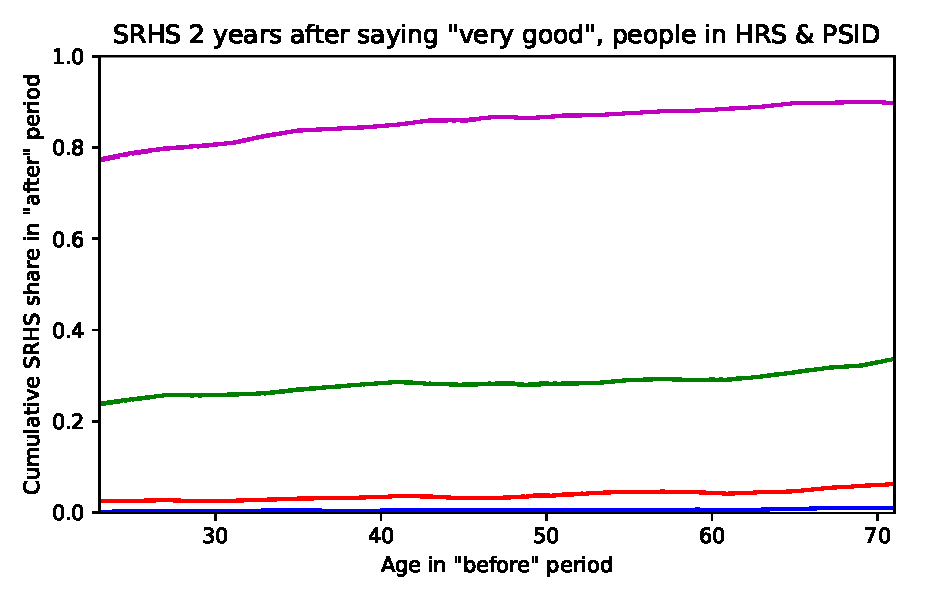
\includegraphics[width=\textwidth]{\FigsDir/TwoStudyOver23AllTransH4T1naiveNoLeg.pdf}
		\caption{One wave ahead}\label{fig:Naive1AheadVeryGood}
	\end{subfigure}
	~
	\begin{subfigure}[b]{0.45\textwidth}
		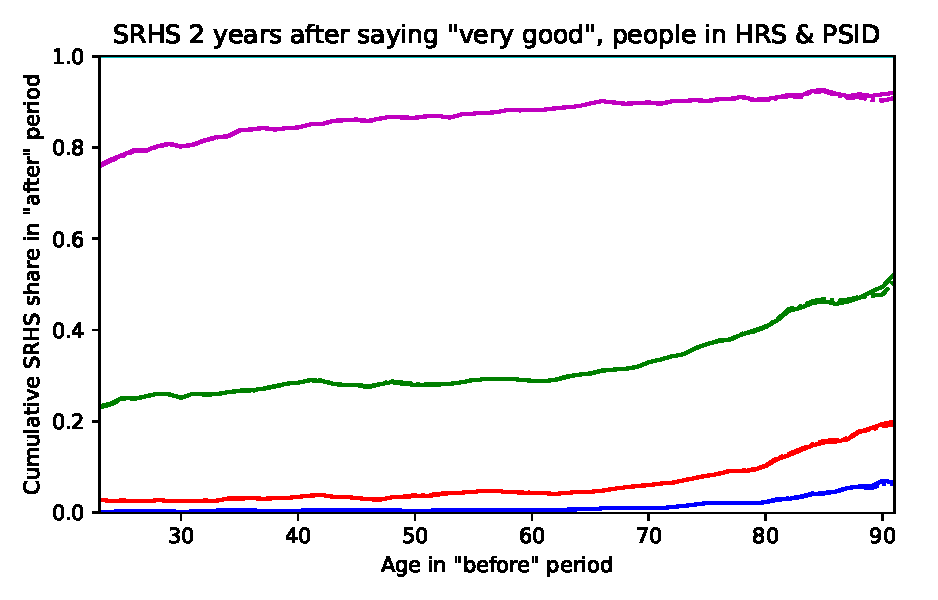
\includegraphics[width=\textwidth]{\FigsDir/TwoStudyOver23AllTransH4T2naiveNoLeg.pdf}
		\caption{Two waves ahead}\label{fig:Naive2AheadVeryGood}
	\end{subfigure}
	
	\begin{subfigure}[b]{0.45\textwidth}
		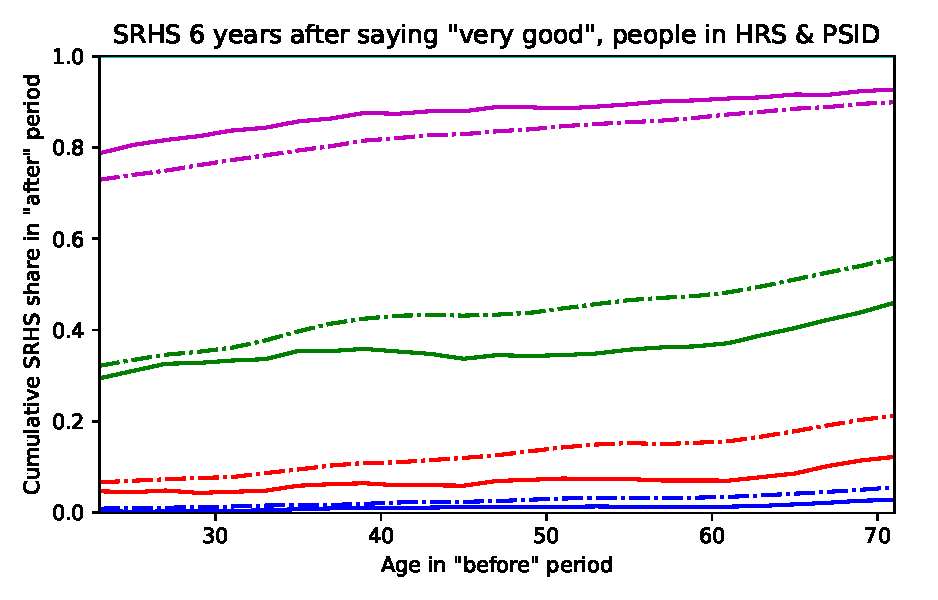
\includegraphics[width=\textwidth]{\FigsDir/TwoStudyOver23AllTransH4T3naiveNoLeg.pdf}
		\caption{Three waves ahead}\label{fig:Naive3AheadVeryGood}
	\end{subfigure}
	~
	\begin{subfigure}[b]{0.45\textwidth}
		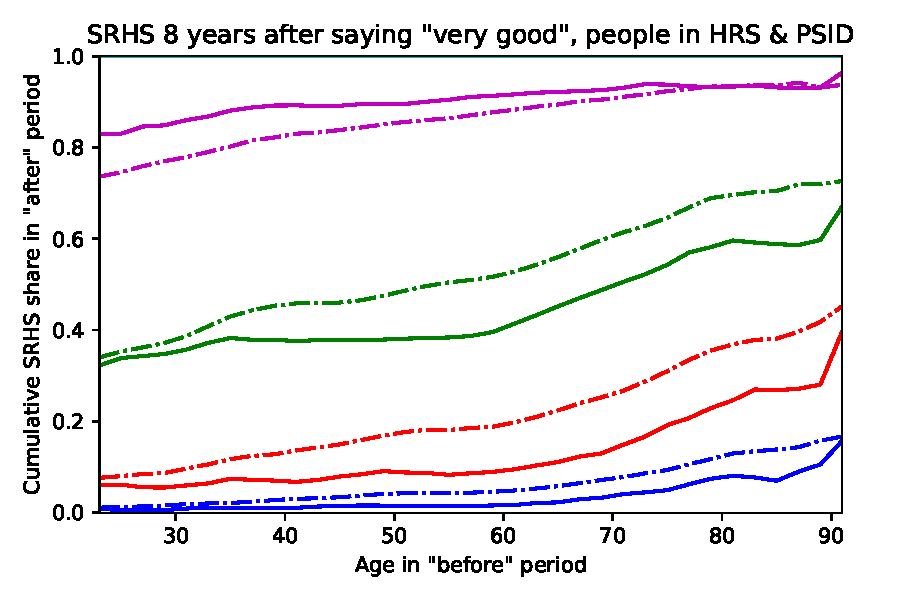
\includegraphics[width=\textwidth]{\FigsDir/TwoStudyOver23AllTransH4T4naiveNoLeg.pdf}
		\caption{Four waves ahead}\label{fig:Naive4AheadVeryGood}
	\end{subfigure}
	
	\begin{subfigure}[b]{0.45\textwidth}
		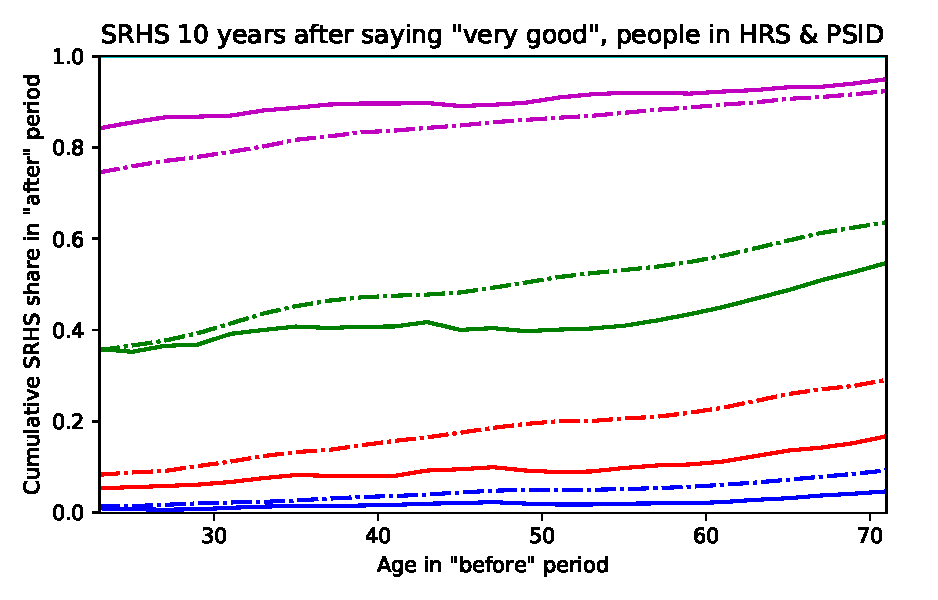
\includegraphics[width=\textwidth]{\FigsDir/TwoStudyOver23AllTransH4T5naiveNoLeg.pdf}
		\caption{Five waves ahead}\label{fig:Naive5AheadVeryGood}
	\end{subfigure}
	~
	\begin{subfigure}[b]{0.45\textwidth}
		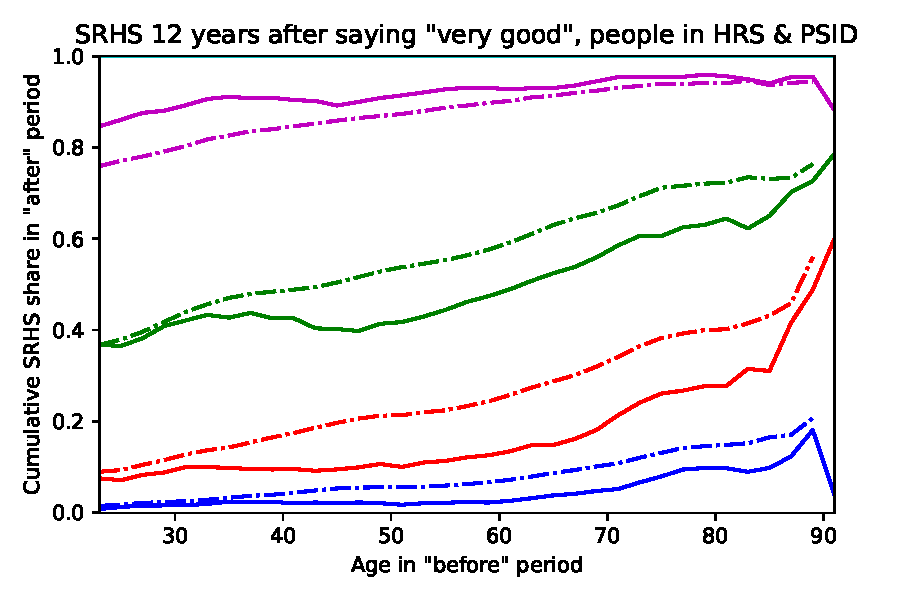
\includegraphics[width=\textwidth]{\FigsDir/TwoStudyOver23AllTransH4T6naiveNoLeg.pdf}
		\caption{Six waves ahead}\label{fig:Naive6AheadVeryGood}
	\end{subfigure}
	\caption{Cumulative distribution of SRHS by age conditional on reporting ``very good'' health in the baseline period in the HRS \& PSID data (solid) vs under simple dynamics (dash-dot).  Predicted distribution from simple dynamics exactly matches the data one wave ahead (by definition), but strongly deviates when projected further in the future.}\label{fig:NaiveTransVG}
\end{figure}

Cursory examination also reveals that one-wave-ahead transition probabilities between healthy and unhealthy SRHS categories do not ``chain up'' correctly: the distribution of SRHS two waves ahead does not agree with the prediction of compounding the one-wave transition probabilities.  For example, 41.9\% of women aged 40-45 who report being unhealthy in the first wave of the MEPS become healthy in the second wave, six months later; women who are already healthy in the first wave have a 94.1\% chance of remaining so.\footnote{Probabilities are nearly identical if transitions from the second wave to the third wave are used instead.}  If SRHS followed a Markov(1) process, then about 36.2\% of women who were unhealthy in wave 1 would also be unhealthy in wave 3.  Instead, however, about 57\% of these women are unhealthy in the third wave, barely lower than the 58.1\% in the second wave.  This continues in subsequent waves: conditional on being unhealthy in wave 1, 53.9\% of women report the same in wave 4, and 52.9\% report being unhealthy in the final wave.  Knowing that someone reported an unhealthy SRHS \textit{two years} prior is almost as valuable for predicting her (binary) SRHS as knowing she reported this \textit{six months} ago.

Using the Panel Study of Income Dynamics (PSID) and Health and Retirement Study (HRS), the same pattern can be seen over the entire life-cycle, and over a longer timespan within each individual.\footnote{Since 1997, the PSID has interviewed its respondents every two years. See Section \ref{sec:Data} for a detailed description of the PSID data used for this short exercise.} I compute simple transition probabilities among the five SRHS categories for respondents between age 23 and 110 from the observed wave-to-wave transitions in the PSID \& HRS, conditional on age and sex, with a two-year wide smoothing kernel.  Figure \ref{fig:NaiveTransVG} plots the empirical distribution of SRHS (conditional on survival) one to six waves after reporting ``very good'' health in the baseline period versus the distribution implied by sequentially applying the age-appropriate simple probabilities, accounting for mortality risk. In the figure, the area below the blue curve represents the proportion of respondents who report poor health, the area between the red and blue curves are those who report fair health, etc. By definition, the one-wave-ahead simple distribution exactly matches the data (Figure \ref{fig:Naive1AheadVeryGood}).  For longer run transitions, however, the simple model predicts too few people reporting ``very good'' health and too many in ``fair'' or ``good'' health; the problem is exacerbated with each successive wave.\footnote{See the Online Appendix for the projected distributions of SRHS from other categories.}

Rather than take SRHS literally, I proffer that a more consistent framework is to interpret SRHS as a noisy signal of a latent health state.  When someone is asked for her SRHS, their true health is projected onto a discrete space of possible replies, subject to reporting error.  That is, there is some partition of the space of ``true health'' and an individual's SRHS represents a noisy report of which subset their health falls in. Moreover, the dynamics of latent health \textit{are} Markov(1), without any dependence on states attained in the past.

Under this interpretation, duration dependence in SRHS arises because many reported transitions among categorical health states are spurious, occurring only due to transitory reporting error rather than genuine changes to health.\footnote{Even without reporting error, some duration dependence would occur: an individual whose most recent shock to true health caused her to \textit{just barely} transition from bad to good health is substantially more likely to transition back to bad health the next period, relative to someone who has reported good health for several consecutive periods because she is far from the boundary.}  Likewise, transition probabilities among categorical health states being nearly identical when observations are taken six months versus two years apart is consistent with true health moving sluggishly (i.e.\ high serial correlation), with reporting shocks driving most changes in SRHS. This process is analogous to the dynamics of household income, which are often modeled as being subject to both permanent and transitory shocks (with measurement error as one source of transitory shock).

In Section \ref{sec:ModelAndEst},  I propose a univariate latent health model as the data-generating process for SRHS. The continuous health state follows an age-dependent AR(1) process, and SRHS is generated through an ordered probit on latent health.  The model can be estimated by maximum likelihood on panel data, calculating the econometrician's belief distribution about each respondent's latent health and updating it after each observation of their SRHS.

The choice to use \textit{reporting} error to account for short run SRHS transitions being inconsistent with longer run transitions, rather than transitory shocks to true health,\footnote{E.g.\ an acute illness, broken bone, or other temporary condition, the interpretation in \cite{Halliday11}.} is motived by \cite{Crossley02}, who find that 28\% of respondents change their SRHS if asked twice in the same interview.  The extent of churn in SRHS before and after taking a relatively short survey about specific health conditions suggests that reporting error is present in SRHS responses. Likewise, the MEPS mails a short survey to respondents after waves 2 and 4 of their panel, the Self-Administered Questionnaire (SAQ), which includes a nearly identical SRHS question. Empirical transition probabilities in the two week span between the MEPS interview and the SAQ are similar to those of a six month gap between interview waves. This fact is inconsistent with SRHS as an accurate representation of health.


\subsection{Related Literature}\label{sec:Lit}

I am not the first to propose latent health as underlying the data-generating process for SRHS. However, this paper is the first to estimate the dynamics of latent health using full information maximum likelihood, explicitly accounting for the econometrician's uncertainty about an individual's true health, and to present comprehensive evidence for the model's ability to fit long-run features of the data.  

In a working paper, \cite{Lange12} employ a two-step method, first recovering the distribution of latent health from self-reports of health outcomes as well as clinical measures, using age-specific static measurement models, then estimating the dynamics of health using the simulated method of moments (SMM).  The second stage estimation uses only one-wave-ahead distributional features as moments to fit, and thus does not account for longer run transitions.  \cite{Halliday11} estimates a dynamic latent health model using SMM to target the distribution of SRHS sequences occurring within several age ranges.  While this approach more fully utilizes the panel structure of the data, it only seeks to fit the frequencies of the three most commonly observed sequences; moreover, no evidence is presented to support the model's ability to accurately predict SRHS transitions.

Other work on SRHS and latent health focuses on particular features of the data or is not concerned with the dynamic process.  \cite{Contoyannis04} address how socioeconomic status affects SRHS transitions, and investigate the extent to which selective attrition might bias estimates of transition probabilities.  A working paper by \cite{Alessie15} augments Dutch panel survey data with administrative health records to construct a univariate health index, which is then also computed for a larger population who are not panel survey respondents; the authors focus on one-wave transitions (annual frequency). \cite{Poterba17} construct a health index using principle component analysis on HRS data, then investigate how this measure affects the stock of wealth as respondents age; they do not estimate dynamics of the health index.

Recent work by \cite{Blundell17} explores whether using several objective measures of health, and potentially a two-factor representation of latent health, provides significant benefit to predicting the timing of retirement, relative to only using SRHS.  The paper focuses on comparing methodologies for estimating labor supply models, rather than constructing a dynamic process for latent health.  The authors write that, ``the literature has interpreted the subjective measures as noisy measures of a single latent health stock.'' While this view may be common in the health literature, it has not received attention among structural modelers.

The observation that SRHS does not follow a Markov(1) process is also not novel.  In recent work, \cite{DeNardi18} propose modeling binary SRHS dynamics as Markov(2), directly accounting for duration dependence by making transition probabilities dependent on the previous period's health state along with its current value. They show that their model is able to reproduce the empirical dynamics of binary SRHS, including the extent of duration dependence and the distribution of the frequency of unhealthy periods across the population.  In Section \ref{sec:Predictions}, I show that the latent health model reproduces the same features targeted in \cite{DeNardi18} and test other model predictions.

The remainder of the paper proceeds as follows.  Section \ref{sec:ModelAndEst} introduces my latent health model and describes how its parameters are identified through maximum likelihood estimation.  Section \ref{sec:Data} describes the two panel datasets that are used to estimate the model, while Section \ref{sec:Results} presents results of the estimation, including a discussion of the model's fit to short- and long-run features of the data. Finally, Section \ref{sec:Conclusion} concludes.


\section{Model \& Estimation}\label{sec:ModelAndEst}

This section presents a univariate latent health model (Section \ref{sec:Model}) and a method for estimating its parameters by maximum likelihood using sequences of SRHS observed in panel data (Section \ref{sec:Estimation}). I discuss how the key parameters are identified by the data in Section~\ref{sec:Identification}.

\subsection{Latent Health Model}\label{sec:Model}

Individual $i$ enters the model at age $\Age_{it}=\AgeMin$ in some discrete time period.  At any time $t$, $i$'s true health status is characterized by his latent health index  $\Health_{it} \in \R$, which is never observed.  However, in a subset of periods after entering the model, the econometrician observes individual $i$'s self-reported health status $\Report_{it} \in \{0,1,\cdots,\TopHealth\}$, with $0$ representing death and each successive value representing a better report.  In the surveys used, these correspond to 1 for ``poor'' up to 5 for ``excellent''.

When an individual of sex $\Sex_i \in \{0,1\}$ enters the model, their initial latent health status is drawn from a normal distribution with mean $\HealthInitMean$ and standard deviation $\HealthInitStd$. Moreover, they are randomly assigned to one of $K$ discrete types according to probabilities $(\TypeProb_1,\cdots,\TypeProb_K)$, which determines the extent of their health reporting error, as standard deviation $\ReportStd_k$.
\begin{equation}\label{HealthInit}
\Age_{it}=\AgeMin \Longrightarrow \Health_{it} \sim N(\HealthInitMean, \HealthInitStd^2), \qquad k_i \sim \text{Discrete}\left((1,\TypeProb_1),\cdots (K,\TypeProb_K) \right).
\end{equation}

In any period in which living individual $i$ is observed, their SRHS $\Report_{it}$ is randomly determined as a linear function of their latent health, subject to a mean zero normal error term and categorical cut points $\Cut = (\Cut_1, \cdots, \Cut_{\TopHealth-1})$.
\begin{equation}\label{Report}
\Report^*_{it} = \LatentParam_0 + \LatentParam_1 \Health_{it} + \ReportShock_{it}, \qquad \ReportShock_{it} \sim N(0,\ReportStd_k^2), \qquad \Report_{it} = 1 + \sum_{\ell = 1}^{\TopHealth-1} \mathbf{1}(\Report^*_{it} \geq \Cut_\ell). 
\end{equation}

Individual $i$'s survival from period $t$ to $t+1$ is determined by a probit on a polynomial of their age and latent health, with a partial interaction for sex:
\begin{equation}\label{Mortality}
\Prob(\Report_{it+1} = 0) = 1 - \Phi(f(\Sex_i,\Age_{it}, \Health_{it})),
\end{equation}
\begin{equation*}
f(\Sex_i,\Health_{it}, \Age_{it}) = \MortParam_0 + \MortParam_\Sex \Sex_i + \MortParam_{\Health1} \Health_{it} + \MortParam_{\Health2} \Health_{it}^2 + (\MortParam_{\Age1} + \MortParam_{\Age\Sex}\Sex_i) \Age_{it} + \MortParam_{\Age2} \Age_{it}^2 + \MortParam_{\Age3} \Age_{it}^3 + \MortParam_{\Health \Age} \Health_{it} \Age_{it}.
\end{equation*}

If $i$ does not die, their latent health in period $t+1$ is drawn from an autoregressive process, subject to a shock with zero mean and unit variance (specified as a mixed normal distribution). Both the correlation coefficient and the auto-regressive level are (transformed) polynomial functions of their age.
\begin{equation}\label{HealthNext}
\Health_{it+1} = \Corr_{\Age} \Health_{it} + (1-\Corr_{\Age}) \ExpHealth_{\Sex\Age} + \HealthShock_{it+1}, ~~~ \HealthShock_{it+1} \sim \text{Mix}((N(\ShockMean_1,\ShockStd_1^2),\MixProb_1), \cdots (N(\ShockMean_L,\ShockStd_L^2),\MixProb_L)),
\end{equation}
\begin{equation*}
\ExpHealth_{\Sex\Age} = \HealthParam_0 + \HealthParam_\Sex \Sex_i + (\HealthParam_1 + \HealthParam_{\Age\Sex} \Sex_i) \Age_{it} + \HealthParam_2 \Age_{it}^2 + \HealthParam_3 \Age_{it}^3 + \HealthParam_4 \Age_{it}^4, ~~~~ \Corr_{\Age} = 1 - 1 \big/ (1 + \exp(\CorrParam_0 + \CorrParam_1 \Age_{it} + \CorrParam_2 \Age_{it}^2 + \CorrParam_3 \Age_{it}^3)).
\end{equation*}
The proportions of the normal mixture are given by the vector of weights $(\MixProb_1,\cdots,\MixProb_L)$, and the corresponding conditional means $\ShockMean_\ell$ and variances $\ShockStd_\ell^2$ are set to generate an overall mean zero and unit variance health shock.

When transitioning from period $t$ to period $t+1$, the individual's age increases by a constant increment $\AgeIncr$ (in years). Let $\Data_i$ represent the set of observations of age-SRHS pairs for individual $i$, and $\Data$ be the collection of all such $\Data_i$.


\subsection{Estimation Method}\label{sec:Estimation}

The latent health model can be estimated using maximum likelihood to identify the values of the model parameters $\ParamVec = (\ShockMean,\ShockStd,\MixProb,\ReportStd,\TypeProb,\LatentParam,\Cut,\MortParam,\HealthParam,\CorrParam)$. Conditional on the parameter values, the econometrician's perceived probability of any particular observation of SRHS at some age depends on all prior observations of the same individual. Indexing the sequence of observations of individual $i$ with $z \in \left\{1,\cdots,Z_i\right\}$, the log probability of observing $\Data_i$ is:
\begin{equation}
\LL_i = \sum_{z=1}^{Z_i} \log \left( \Prob \left(\Report_{iz} ~\big|~ \Age_{iz}, \Report_{iz-1}, \Age_{iz-1},\cdots \Report_{i1},\Age_{i1}, \Delta \right) \right) .
\end{equation}
 The overall log likelihood of the parameter vector $\ParamVec$ given data $\Data$ is the sum across each individual's log likelihood contribution:
\begin{equation}
\mathcal{L}(\ParamVec~|~\Data) = \sum_{i=1}^{I} \LL_i.
\end{equation}

To calculate the probability of any one observation, the econometrician must take into account the distribution over the individual's current latent health $\Health_{it}$ and their possible reporting error type $k_i$, given all prior observations and their current age. Suppose this distribution is characterized by the type-conditional probability distribution functions $(g_1(\Health), \cdots, g_K(\Health))$ and corresponding type probabilities $(\TypeProbPcvd_1,\cdots, \TypeProbPcvd_K)$. The probability of observing a particular categorical health report for a living individual is then:
\begin{equation}\label{ReportProb}
\Prob \left( \Report_{iz} ~\big|~ \left\{\TypeProbPcvd_k \right\}, \left\{g_k(\cdot) \right\} \right) = \sum_{k=1}^K \TypeProbPcvd_k \int_{-\infty}^{\infty} \bigg[ \underbrace{\Phi \left(\frac{\Cut_{\Report} - \LatentParam_0 - \LatentParam_1 \Health}{\ReportStd_k} \right) - \Phi \left(\frac{\Cut_{\Report-1} - \LatentParam_0 - \LatentParam_1 \Health}{\ReportStd_k} \right)}_{= \Prob(\Report_{iz} ~|~ \Health_{iz} = \Health, ~ \sigma_i=\ReportStd_k)} \bigg]  g_k(\Health) d \Health.
\end{equation}
The top and bottom cut points $\Cut_K$ and $\Cut_0$ are simply $\pm \infty$, representing a one-sided interval.

To aid in the computation of such probabilities, the range of latent health values that individuals can reasonably attain under parameters $\Delta$ is discretized into $N$ intervals, and then replicated by the number of types $K$.  When calculating the likelihood of individual $i$'s observed sequence of SRHS, I represent the econometrician's distribution over $i$'s latent health and reporting type as a stochastic vector denoted $\HealthDstnPcvd_i$, a discretization of both $(\TypeProbPcvd_1,\cdots,\TypeProbPcvd_K)$ and $(g_1,\cdots,g_K)$.

When individuals enter the model at age $\AgeMin$, the econometrician's discretized distribution over the unobserved variables can be constructed using $\HealthInitMean$ and $\HealthInitStd$ and the type probabilities $\TypeProb = (\TypeProb_1,\cdots,\TypeProb_K)$. Denoting the cut points of the discretization as $\{\DiscreteCut_n\}_{n=0}^N$, the initial distribution of unobserved variables at model entry for each sex is:\footnote{For all specifications, I used $N=120$ evenly spaced intervals on $[-12,28]$, censoring well under one millionth of the population at any age-- usually orders of magnitude less. With $K=3$ reporting error types, the discretization of unobserved variables has 360 nodes. When computing transition probabilities, I treat the topmost and bottommost discrete cuts as $\DiscreteCut_0,\DiscreteCut_N=\pm \infty$ so that all probability mass is accounted for.}
\begin{equation}
\HealthDstn_{\AgeMin}(\Sex,k,n) = \TypeProb_k \left(\Phi((\DiscreteCut_n - \HealthInitMean)/\HealthInitStd) - \Phi((\DiscreteCut_{n-1} - \HealthInitMean)/\HealthInitStd) \right) ~~\text{for}~ s=0,1; ~~ k=1,\cdots,K; ~~ n=1,\cdots,N.
\end{equation}

The vast majority of respondents in the data are not immediately observed upon model entry, but instead first appear in the data later in life, after being exposed to a sequence of health shocks and surviving all mortality shocks to that point. To calculate the econometrician's discretized distribution over unobserved variables \textit{just before} first observing someone who has lived to age $\Age > \AgeMin$, I construct two additional arrays.

First, for each age between $\AgeMin$ and the highest age observed in the data $\AgeMax$, $\LivPrb_\Age$ is a $2 \times KN$ array of survival probabilities from age $\Age$ to $\Age + \AgeIncr$ on the discretized space using \eqref{Mortality}:
\begin{equation}
\LivPrb_\Age(\Sex,k,n) = \Phi(-f(\Sex,(\DiscreteCut_n+\DiscreteCut_{n-1})/2, \Age) ~~\text{for}~ s=0,1; ~~ k=1,\cdots,K; ~~n=1,\cdots,N; ~~ \Age=\AgeMin,\AgeMin+\AgeIncr,\cdots,\AgeMax.
\end{equation}
Second, the $2 \times N \times N$ survival-conditional Markov transition matrix $\TransPrb_\Age$ among discretized latent health states from age $\Age$ to $\Age + \AgeIncr$ is constructed using the autoregressive parameters $\CorrParam$, expected health parameters $\HealthParam$, and health shock distibution parameters $(\MixProb,\ShockMean,\ShockStd)$:
\begin{equation}
\TransPrb_\Age(\Sex,n,n') = \sum_{\ell=1}^L \MixProb_\ell \left[ \Phi \left( \frac{\DiscreteCut_{n'} - \ShockMean_\ell - \Corr_{\Age} \hat{\Health}_n - (1-\Corr_{\Age})\ExpHealth_{\Sex\Age}}{\ShockStd_\ell} \right) - \Phi \left( \frac{\DiscreteCut_{n'-1} - \ShockMean_\ell - \Corr_{\Age} \hat{\Health}_n - (1-\Corr_{\Age})\ExpHealth_{\Sex\Age}}{\ShockStd_\ell} \right) \right]
\end{equation}
\begin{equation*}
\text{for}~~s =0,1; ~~~ n=1,\cdots,N; ~~~ n'=1,\cdots,N; ~~~ \Corr_{\Age} ~\text{and}~ \ExpHealth_{\Sex\Age} ~\text{as given in \eqref{HealthNext}}; ~~~ \hat{\Health}_n = \frac{\DiscreteCut_n + \DiscreteCut_{n-1}}{2}.
\end{equation*}
Conditional on sex, $\TransPrb_\Age(\Sex)$ can be replicated $K$ times along the (block) diagonal of a $KN \times KN$ matrix denoted $\overline{\TransPrb}_\Age(\Sex)$, which is filled with zero on its off-diagonal blocks. This larger Markov matrix represents the overall transition probabilities among discretized unobserved variables from one age to the next.

The discretized distribution of latent health $\Health$ and reporting error type $k$ at all subsequent ages, conditional on surviving to that age, can then be constructed using $\LivPrb_\Age$ and $\overline{\TransPrb}_\Age$ by iterating over age and sex according to:\footnote{The Hadamard product (circle-dot) represents element-wise multiplication.}
\begin{equation}
\HealthDstn_{\Age + \AgeIncr}(\Sex) = \left[ (\HealthDstn_{\Age}(\Sex) \odot \LivPrb_\Age(\Sex)) / (\HealthDstn_{\Age}(\Sex) \cdot \LivPrb_\Age(\Sex)) \right] \times \overline{\TransPrb}_{\Age}(\Sex) ~~\text{for}~ \Sex=0,1; ~~ \Age = \AgeMin, \AgeMin+\AgeIncr, \cdots, \AgeMax-\AgeIncr.
\end{equation}
The factor in brackets represents the distribution of latent health (and reporting error type) among individuals who do not die at the end of age $\Age$, just before the latent health transition occurs; post-multiplying by the Markov matrix for discretized health for this sex executes that transition. For an individual who is first observed in the data at age $\Age$, $\HealthDstn_\Age(s)$ represents the econometrician's distribution over their unobserved variables. In terms of the probability of observing a particular value of SRHS in \eqref{ReportProb}, $\HealthDstn_\Age(s)$ is a discretized representation of $(\TypeProb_1,\cdots,\TypeProb_K)$ and $(g_1,\cdots,g_K)$, conditioning on the fact that a person of this sex has survived.

To compute the term in brackets inside the integral in \eqref{ReportProb}, I construct a $H \times KN$ matrix of reporting probabilities $\ReportPrb$ using the latent parameters $\LatentParam$ and the cut points $\Cut$:
\begin{equation}
\ReportPrb(\Report,k,n) = \Phi \left(\frac{\Cut_{\Report} - \LatentParam_0 - \LatentParam_1 \hat{\Health}_n}{\ReportStd_k} \right) - \Phi \left(\frac{\Cut_{\Report-1} - \LatentParam_0 - \LatentParam_1 \hat{\Health}_n}{\ReportStd_k} \right)
\end{equation}
\begin{equation*}
\text{for}~~x = 1,\cdots,H; ~~~ k=1,\cdots,K; ~~~ n=1,\cdots,N; ~~~ \text{and}~~ \hat{\Health}_n = \frac{\DiscreteCut_n + \DiscreteCut_{n-1}}{2}.
\end{equation*}
The element $\ReportPrb(\Report,k,n)$ represents the probability that an observed individual of reporting error type $k$ will report SRHS of $\Report_{it}=x$ if their latent health is in the $n$th interval.  Note that reporting probabilities do not depend on age nor sex. If the econometrician's distribution over unobserved variables is currently $\HealthDstnPcvd_{i}$, then the probability of $i$ reporting their categorical health as $\Report_{it}$ is simply $\HealthDstnPcvd_{i} \cdot \ReportPrb(\Report_{it})$; this reduces right-hand side of \eqref{ReportProb} to a mere vector product.

To calculate the contribution to log likelihood from individual $i$'s sequence of SRHS, I begin by initializing the distribution of $i$'s unobserved variables $\HealthDstnPcvd_{i}$ to the distribution $\HealthDstn_{\Age}(\Sex_i)$ for the first age at which they are observed-- the prior distribution of their latent health under parameters $\ParamVec$ given that $i$ has survived to this age.  I also initialize $\LL_i$ to zero, and the ``cumulative survival probability'' $\CumLivPrb_i$ is set at one, representing the probability that $i$ has not died since the last observation incorporated into $\LL_i$.

From these initial conditions, I iterate over time $t$. If $i$ is observed alive at time $t$, then $\CumLivPrb_i$ is incorporated into $\LL_i$ and reset to one; if $i$ is reported as dead ($\Report_{it} = 0$), the additive complement of $\CumLivPrb_{i}$ is accumulated into $\LL_i$ and its computation is complete.
\begin{equation}\label{LivPrbLL}
\LL_i := \begin{cases}
\LL_{i} + \log(\CumLivPrb_i) & \text{if } \Report_{it} \geq 1 \\
\LL_{i} + \log(1 - \CumLivPrb_i) & \text{if } \Report_{it} = 0 \\
\end{cases}, \qquad \CumLivPrb_i := 1.
\end{equation}
Next, the probability of $i$ reporting $\Report_{it}$ (given the econometrician's distribution $\HealthDstnPcvd_{i}$) is accumulated into $\LL_i$, and the econometrician's distribution is updated using Bayes' rule:
\begin{equation}\label{ReportPrbLL}
\LL_i := \LL_i + \log(\HealthDstnPcvd_{i} \cdot \ReportPrb(\Report_{it})), \qquad \HealthDstnPcvd_{i} := (\HealthDstnPcvd_{i} \odot \ReportPrb(\Report_{it})) / (\HealthDstnPcvd_{i} \cdot \ReportPrb(\Report_{it})).
\end{equation}
If $\Report_{it}$ is not observed this period (e.g.\ because $i$ was not surveyed or refused to answer), then both \eqref{LivPrbLL} and \eqref{ReportPrbLL} are skipped.

To move individual $i$ to period $t+1$, I incorporate the survival probability into $\CumLivPrb_{i}$, then update the  distribution $\HealthDstnPcvd_{i}$ using survival probabilities $\LivPrb_\Age(\Sex_i)$ and the Markov matrix $\overline{\TransPrb}_\Age(\Sex_i)$:
\begin{equation}\label{NextPrdLL}
\CumLivPrb_i := \CumLivPrb_i (\HealthDstnPcvd_{i} \cdot \LivPrb_\Age(\Sex_i)), \qquad \HealthDstnPcvd_{i} := \left[ (\HealthDstnPcvd_{i} \odot \LivPrb_\Age(\Sex_i)) / (\HealthDstnPcvd_{i} \cdot \LivPrb_\Age(\Sex_i)) \right] \times \overline{\TransPrb}_\Age(\Sex_i), \qquad \Age_i := \Age_i + \AgeIncr.
\end{equation}
The steps in \eqref{LivPrbLL}, \eqref{ReportPrbLL}, and \eqref{NextPrdLL} are then repeated until the last observation of $i$ is included in $\LL_i$, incorporating all $Z_i$ reports of categorical health (including an observed death).

To estimate the model, I maximize the log likelihood function using the Broyden-Fletcher-Goldfarb-Shanno algorithm with many restarts. The covariance matrix is calculated using the Huber sandwich estimator, so the standard errors are robust to model misspecification.


\subsection{Identification}\label{sec:Identification}

The model generates observed health reports $\Report_{it}$ from a latent variable $\Report^*_{it}$ based on another latent variable, the true health index $\Health_{it}$.  The level of these latent variables is thus unidentified, so I assume that $\LatentParam_0=0$ and $\Cut_1=0$.  Having latent health of \textit{exactly} zero means that an individual would report the lowest category of SRHS (``poor'') with probability one half, and some higher category the other half of the time.  Because the health shock $\HealthShock$ is assumed to have unit variance, the scale of latent health $\Health_{it}$ can be interpreted as the number of standard deviations (of one period's health shock) away from this benchmark level.

The reporting shocks $\ReportShock_{it}$ are mean zero and normally distributed for all reporting types $k$, but the scale of $\Report_{it}^*$ would be indeterminate without the normalizing assumption that the overall distribution of reporting errors has unit variance. With mean zero type-conditional shock distributions, this requires imposing the condition:\footnote{In the estimation, this condition means that the reporting error variance for one of the types is strictly determined by the others, just as the proportion $\TypeProb_k$ for one type is determined by the others because the fractions must sum to 1.}
\begin{equation}
\sum_{k=1}^K \TypeProb_k \ReportStd_k^2 = 1.
\end{equation}

Temporarily setting aside heterogeneity in $\ReportStd$, the normalized unit variance of reporting shocks means that the parameter $\LatentParam_1$ represents how informative SRHS is about latent health. That is, a large value of $\LatentParam_1$ (and correspondingly large scale of the SRHS cut points $\Cut$) means that an individual's reported health status is likely to be an accurate portrayal of his latent health, rather than arising from mere reporting error. When the cut points are far apart, the unit variance $\ReportShock$ shocks are less likely to cross one or more of them.

The primary identification challenge for the latent health model is to separate the autocorrelation process of latent health from the noise of reporting error in SRHS.  Holding $\LatentParam_1$ fixed, lower values of $\Corr_\Age$ (from lower $\CorrParam$ parameters) are associated with more period-to-period changes in SRHS; as $\Corr_\Age$ approaches zero, both latent health and SRHS would approach being random draws from population health.  Likewise, holding the $\CorrParam$ parameters fixed, a smaller $\LatentParam_1$ would also generate more volatility in SRHS, approaching iid draws as $\LatentParam_1$ approaches zero, because SRHS would represent pure noise.  From the perspective of one-wave transitions in SRHS, these parameters are not separately identified: there is a locus of $\Corr_\Age$ and $\LatentParam_1$ that would generate nearly identical wave-to-wave transitions.

The resolution of this problem lies in the dynamics of SRHS beyond one-wave-ahead transitions.  If autocorrelation in latent health is relatively high and the information value of SRHS is low (small $\LatentParam_1$), then short run changes in SRHS largely represent reporting error.  Conditional on SRHS in the reference period, the distribution of SRHS \textit{two} waves ahead will be very similar to its distribution \textit{one} wave ahead, as true latent health did not change much.  Conversely, if the observed distribution of one period changes in SRHS arose from relatively low autocorrelation of $\Health$ and higher $\LatentParam_1$, then these transitions do reflect true changes in latent health.  Consequently, the distribution of latent health would change further after two transitions, and these changes would be accurately reflected by SRHS, resulting in a \textit{less similar} two-wave-ahead distribution of SRHS compared to the prior case.

The maximum likelihood estimation thus identifies persistent changes in latent health from transitory reporting error by finding parameters that best match the wave-to-wave dynamics of SRHS as well as longer run transitions.  A key benefit of MLE over approaches that target a specific set of data moments to fit (such as the simulated method of moments) is that it naturally incorporates all of the SRHS transitions into the objective function. The previous paragraphs use one- and two-wave-ahead transitions to provide intuition for the separate identification of signal and noise in SRHS, but MLE utilizes all observed transitions for the entire span of the dataset used.

In the panel data described in Section \ref{sec:Data}, volatility in SRHS is not homogeneous across sample respondents. Some individuals are much more consistent about reporting the same (or adjacent) SRHS, while a small proportion of respondents' health reports are extremely variable, frequently changing by multiple categories in consecutive waves. Model specifications without heterogeneity in the magnitude of reporting shocks $\ReportStd$ significantly under-predict the fraction of respondents who would report the same SRHS over several consecutive waves (see Online Appendix). The standard deviation of reporting shocks for each type $\ReportStd_k$ and the proportions of each type $\TypeProb_k$ are thus identified through this heterogeneity in SRHS volatility.

Likewise, a basic specification that models shocks to latent health $\HealthShock$ as standard normal does not match some features of the data. Even when fitting the overall distribution of SRHS by age (i.e.\ the trend in latent health), the data show more large jumps from a high SRHS category to one multiple steps below than vice versa. Moreover, these changes are persistent, indicating a true change in latent health rather than reporting error. A negatively skewed distribution with significant excess kurtosis better fits this pattern than the basic assumption of symmetrically distributed shocks to latent health. The means, standard deviations, and mixture weights of the latent health shocks ($\ShockMean_\ell$, $\ShockStd_\ell$, and $\MixProb_\ell$ respectively) are identified by asymmetries in changes to latent health.\footnote{In the specifications presented in the paper, I use $L=2$, so only $\ShockMean_1$, $\ShockStd_1$, and $\MixProb_1$ are structurally estimated. Their analogues for $\ell=2$ are strictly determined by the normalization of zero mean, unit variance shocks.} 

Identification of the remaining parameters is straightforward and does not require extended discussion: the frequency of death by age and health identifies the mortality parameters $\MortParam$, the cross-sectional distribution of SRHS identifies the cut points $\Cut$ (conditional on the scale of latent health and $\LatentParam_1$), changes in the distribution of SRHS by age identify the expected health parameters $\HealthParam$, etc.  It is worth noting, however, that the key identification arguments presented above are bolstered by the inclusion of more than two categories of SRHS (i.e.\ ``healthy'' and ``unhealthy''), as there is more information about the magnitude of a reported change in health.


\section{Data}\label{sec:Data}

The latent health model presented in Section \ref{sec:ModelAndEst} could be estimated on any panel dataset that includes SRHS and has at least three data waves per respondent.\footnote{Not all respondents must appear in at least three waves, but model identification requires that at least some individuals are observed three or more times; see Section \ref{sec:Identification}.}  In this paper, I apply the model to a dataset that combines two well known surveys of American households: the Health and Retirement Study (HRS) and the Panel Study of Income Dynamics (PSID). This section provides an overview of the sample selection method, summarized in Table \ref{table:DataSummary}.

\begin{table}[ht]
\normalsize
\begin{center}
\caption{Dataset Summary Statistics by Specification}\label{table:DataSummary}
\newsavebox{\DataSummaryBox}
\sbox{\DataSummaryBox}{  
\begin{tabular}{ccccccccrrcc}
\hline \hline

\rule{0pt}{2.5ex} Data & Sex & Start & End & Freq & $\underline{j}$ & $\overline{j}$ & $\hat{j}$ & \multicolumn{1}{c}{Inds} & \multicolumn{1}{c}{Obs} & \multicolumn{1}{c}{Deaths} & \multicolumn{1}{c}{5+ obs?} \\
\hline
%MEPS & F & 1996 & 2016 & 6 mo & 18 & 86.5 & 0.5 & 126,486 & 601,713 & 1,168 & 89.5\% \\
%MEPS & M & 1996 & 2016 & 6 mo & 18 & 86.5 & 0.5 & 110,044 & 518,577 & 1,314 & 87.7\%  \\
HRS & F & 1996 & 2016 & 2 yr & 50 & 115 & 1.0 & 20,108 & 107,542 & 5,794 & 50.1\% \\
HRS & M & 1996 & 2016 & 2 yr & 50 & 115 & 1.0 & 16,094 & 81,091 & 5,286 & 46.7\%  \\
PSID & F & 1997 & 2017 & 2 yr & 23 & 110 & 1.0 & 11,787 & 69,329 & 1,012 & 55.6\%  \\
PSID & M & 1997 & 2017 & 2 yr & 23 & 110 & 1.0 & 10,791 & 58,316 & 995 & 50.0\% \\
% Mixed & F & 1996 & 2017 & varies & 18 & 115 & 1.0 & 120,720 & 343,461 & 6,918 & 13.4\%  \\
% Mixed & M & 1996 & 2017 & varies & 18 & 115 & 1.0 & 102,965 & 281,681 & 6,568 & 12.3\% \\
\hline
\rule{0pt}{2.2ex}Both & * & 1996 & 2017 & 2 yr & 23 & 115 & 1.0 & 58,635 & 324,646 & 12,896 & 52.3\% \\
\hline\hline
\end{tabular}
} 
\usebox{\DataSummaryBox}  
\settowidth\TableWidth{\usebox{\DataSummaryBox}} % Calculate width of table so notes will match  
\vspace{0.0cm} \parbox{\TableWidth}{
\begin{flushleft}
	\textbf{NB:} Observation counts from individual lines do not sum to the bottom row because the combined data includes HRS respondents younger than 50, but the HRS specifications (in the Online Appendix) begin at this age.
\end{flushleft}
}
\end{center}
\end{table}


The PSID data includes Americans of all ages, while the HRS focuses only on the older population-- those approaching and beyond retirement age. I combine the two panel surveys into a single dataset in order to sharply identify both health dynamics among the working age population (which the HRS lacks) and the mortality process by age and health (as the PSID has relatively few deaths). Specifications estimated on each panel survey independently are provided in the Online Appendix.\footnote{The model has also been estimated using on MEPS data, which has many more respondents, but a much shorter panel for each.} The combined dataset includes over 58,000 individuals and almost 325,000 observations of SRHS, plus nearly 13,000 observed deaths.

The surveys elicit SRHS using slightly different wording, presented in each subsection below.  However, both surveys have the same five categorical responses for SRHS: poor, fair, good, very good, and excellent.  Nonresponse to SRHS questions due to refusal or ``not knowing'' is very low, under 0.3\%, and is not correlated with prior health status (nor later reports).  Attrition from the surveys for reasons other than death is likewise not predicted by SRHS; mortality itself is accounted for by the model.

Both the HRS and PSID construct their samples to be representative of the U.S.\ population, and I use the provided respondent weights to adjust contributions to the log likelihood function.  These weights are normalized to have a mean of one, to preserve the relative magnitude of the likelihood function (which is relevant when computing standard errors using its Hessian). The distribution of SRHS by age and sex closely matches across the two datasets for the range of ages in which they overlap.



\subsection{HRS Data}\label{sec:HRS}

The primary sample population for the HRS includes only Americans older than 50.\footnote{Spouses and other household members of the originally selected individual are also included as HRS respondents, even if they are 50 or younger.}  The HRS focuses on labor supply, medical events, health status, and assets as its respondents transition from working life and into retirement.  Primary respondents enter the HRS sample between ages 51 and 57, and then are interviewed every two years until their death.  The sample is refreshed every six years (three waves) with a cohort of newly eligible households.  The survey began in 1992 and was merged with its sister project, Assets and Health Dynamics Among the Oldest Old (AHEAD), in 1998; the dataset for this paper uses the 1996-2016 waves of the HRS. The SRHS question in the HRS asks, ``Would you say your health is excellent, very good, good, fair, or poor?"

Whether as spouses or children (or other dependents), individuals of all ages are found in the HRS, but the data is increasingly sparse at ages below the primary sample eligibility age of 51.  I drop the extremely few respondents who would first enter the data older than 95, so the highest age that has to be considered ($\AgeMax$, in the notation of Section \ref{sec:Model}) is 115 (but no one attains it). The vast majority of life-cycle models use one year discrete periods, including many that are estimated on two-year panel data like the HRS or PSID (post-1997).  To follow this convention, I set the age increment to one year, inserting a missing SRHS observation for each individual in the ``pseudo wave'' for each odd-numbered year.

The HRS dataset for estimation includes about 36,000 individuals and nearly 190,000 person-wave observations of SRHS. There is no dearth of death in the HRS: over 11,000 of the sample individuals (nearly one third) are observed to die, allowing fairly sharp identification of the mortality process.  Just under half of the individuals from the HRS data are observed alive for at least five waves; the vast majority of the remainder joined the HRS too late to be observed fives times (i.e.\ they are in the cohorts added in 2010 and 2016) or have died, with very little attrition for other reasons.


\subsection{PSID Data}\label{sec:PSID}

The PSID began in 1968 with a representative sample of American households.  Household members were interviewed every year until 1997, when the survey switched to a biannual format. The PSID famously uses a snowballing sample, with new respondents added as original sample members marry, form their own households, and reproduce; the survey population has also been occasionally refreshed with recent immigrant households to maintain representativeness.  Once included in the primary sample, the survey follows an individual and their descendants until death.

The PSID's SRHS question asks, ``Would you say your health in general is excellent, very good, good, fair, or poor?''  While all sample household members have some individual-level data in the PSID, SRHS is only elicited for the head and spouse; the health status of other members is only measured with a binary variable.  My dataset thus only includes observations of individuals who are a household head or spouse in that particular wave. The PSID has included a SRHS question since 1984, but I restrict my dataset to the 1997 to 2017 waves, beginning with the switch to two-year waves.

The PSID considers most college students to be dependents of their parents' household, rather than heads of newly formed households.  Even in the late teens and early twenties, health is already correlated with education, so the PSID data are not representative of the full population.  In fact, the cross-sectional distribution of SRHS rapidly shifts toward better categories between age 18 and 25, but this is merely an artifact of the shifting sample population as college graduates become household heads. To (mostly) avoid this issue, I drop observations younger than 23, when most graduates have already split off from their original household.\footnote{As with the HRS, I also drop the handful of respondents who would enter the data older than 90.} The age at model entry is set at $\AgeMin=23$ to match this data cut.\footnote{Many dynamic structural models of lifecycle decision-making also have their agents begin at age 22 to 25, so that educational attainment can be treated as exogenous. Given that the intent of this is work to provide more realistic health dynamics for such models, this truncation of the data is appropriate.}

The PSID contributes about 22,600 individuals and 127,000 observations of SRHS.  Because the PSID data includes adults of any age, not just older individuals, only about 2,000 deaths are observed over twenty years. Over half half of the PSID respondents in my data are observed alive for at least five waves, and about 22\% are observed in all eleven waves.  However, just under one third of sample individuals appear for only one or two waves.  These respondents might have qualified as a ``wife'' under the PSID's standard for cohabiting partners, then subsequently broke off their relationship and were no longer tracked.


\section{Results}\label{sec:Results}

I now present and discuss estimated parameters of the latent health model (Section~\ref{sec:Parameters}) disciplined on HRS and PSID data, including its ability to match short- and long-run SRHS transitions (Section~\ref{sec:Fit}).\footnote{Results for specifications using one dataset at a time are presented in the Online Appendix.} Other latent health model predictions are tested in Section~\ref{sec:Predictions}.

\subsection{Parameter Estimates}\label{sec:Parameters}

Estimated parameters and standard errors are shown in Table \ref{tab:TwoStudyTable}, for specifications with men and women separately, as well as both sexes together. Across specifications, almost all standard errors are an order of magnitude smaller than the point estimates, indicating fairly sharp identification of the model parameters.  The only exceptions are the interaction coefficients for mortality, which are on the edge of being significantly different from zero.

\begin{table}
\tiny
\singlespace
\begin{center}
\caption{Paramaters Estimated by Maximum Likelihood on HRS and PSID Data}\label{tab:TwoStudyTable}
\newsavebox{\TwoStudyTableBox}
\sbox{\TwoStudyTableBox}{  
\begin{tabular}{clccc}
\hline \hline
\rule{0pt}{2.5ex}Param & \multicolumn{1}{c}{Description} & Women & Men & All \\
\hline
\rule{0pt}{2.2ex}$\theta_{0}'$ & Mortality probit: level at model start $\underline{j}$ & 2.632 & 2.222 & 2.565 \\
\rule{0pt}{2.2ex} & & (7.81e-2) & (7.94e-2) & (5.31e-2) \\
\rule{0pt}{2.2ex}$\theta_{s}$ & Mortality probit: shifter for men & 0.00 & 0.00 & -0.273 \\
\rule{0pt}{2.2ex} & & (---) & (---) & (2.79e-2) \\
\rule{0pt}{2.2ex}$\theta_{h1}'$ & Mortality probit: first derivative w.r.t health at $\Health=0$ & 0.136 & 0.139 & 0.137 \\
\rule{0pt}{2.2ex} & & (1.03e-2) & (1.19e-2) & (7.83e-3) \\
\rule{0pt}{2.2ex}$\theta_{h2}'$ & Mortality probit: second derivative w.r.t health at $\Health=0$ & -6.77e-3 & -5.14e-3 & -5.99e-3 \\
\rule{0pt}{2.2ex} & & (1.02e-3) & (1.17e-3) & (7.55e-4) \\
\rule{0pt}{2.2ex}$\theta_{j1}'$ & Mortality probit: first derivative w.r.t age at $\underline{j}$ & -1.50e-2 & -4.04e-3 & -1.09e-2 \\
\rule{0pt}{2.2ex} & & (3.30e-3) & (3.23e-3) & (1.56e-3) \\
\rule{0pt}{2.2ex}$\theta_{j2}'$ & Mortality probit: second derivative w.r.t age at $\underline{j}$ & 2.25e-4 & -2.53e-4 & 3.20e-5 \\
\rule{0pt}{2.2ex} & & (1.33e-4) & (1.35e-4) & (3.00e-6) \\
\rule{0pt}{2.2ex}$\theta_{j3}'$ & Mortality probit: third derivative w.r.t age at $\underline{j}$ & -2.82e-5 & -1.69e-5 & -2.36e-5 \\
\rule{0pt}{2.2ex} & & (3.54e-6) & (4.00e-6) & (1.18e-6) \\
\rule{0pt}{2.2ex}$\theta_{hj}$ & Mortality probit: coefficient on age$\times$health & -2.14e-4 & -2.57e-4 & -2.31e-4 \\
\rule{0pt}{2.2ex} & & (1.11e-4) & (1.43e-4) & (8.91e-5) \\
\rule{0pt}{2.2ex}$\theta_{js}$ & Mortality probit: coefficient on age, adjustment for men & 0.00 & 0.00 & 9.69e-4 \\
\rule{0pt}{2.2ex} & & (---) & (---) & (3.40e-4) \\
\hline
\rule{0pt}{2.2ex}$\gamma_{0}'$ & Correlation factor: level at model start $\underline{j}$ & 3.216 & 3.110 & 3.119 \\
\rule{0pt}{2.2ex} & & (0.136) & (0.163) & (9.87e-2) \\
\rule{0pt}{2.2ex}$\gamma_{j1}'$ & Correlation factor: first derivative w.r.t age at $\underline{j}$ & 8.68e-2 & 6.89e-2 & 8.25e-2 \\
\rule{0pt}{2.2ex} & & (1.36e-2) & (1.71e-2) & (1.02e-2) \\
\rule{0pt}{2.2ex}$\gamma_{j2}'$ & Correlation factor: second derivative w.r.t age at $\underline{j}$ & -5.45e-3 & -3.69e-3 & -4.85e-3 \\
\rule{0pt}{2.2ex} & & (8.32e-4) & (1.06e-3) & (6.36e-4) \\
\rule{0pt}{2.2ex}$\gamma_{j3}'$ & Correlation factor: third derivative w.r.t age at $\underline{j}$ & 1.53e-4 & 1.03e-4 & 1.35e-4 \\
\rule{0pt}{2.2ex} & & (2.32e-5) & (2.90e-5) & (1.78e-5) \\
\hline
\rule{0pt}{2.2ex}$\beta_{0}'$ & Expected health: level at model start $\underline{j}$ & 10.668 & 12.049 & 11.061 \\
\rule{0pt}{2.2ex} & & (0.688) & (0.798) & (0.512) \\
\rule{0pt}{2.2ex}$\beta_{s}$ & Expected health: shifter for men & 0.00 & 0.00 & 0.928 \\
\rule{0pt}{2.2ex} & & (---) & (---) & (0.186) \\
\rule{0pt}{2.2ex}$\beta_{j1}'$ & Expected health: first derivative w.r.t age at $\underline{j}$ & -0.846 & -0.996 & -0.913 \\
\rule{0pt}{2.2ex} & & (0.117) & (0.136) & (8.77e-2) \\
\rule{0pt}{2.2ex}$\beta_{j2}'$ & Expected health: second derivative w.r.t age at $\underline{j}$ & 5.50e-2 & 6.46e-2 & 6.05e-2 \\
\rule{0pt}{2.2ex} & & (9.63e-3) & (1.10e-2) & (7.20e-3) \\
\rule{0pt}{2.2ex}$\beta_{j3}'$ & Expected health: third derivative w.r.t age at $\underline{j}$ & -1.93e-3 & -2.36e-3 & -2.15e-3 \\
\rule{0pt}{2.2ex} & & (3.38e-4) & (3.90e-4) & (2.54e-4) \\
\rule{0pt}{2.2ex}$\beta_{js}$ & Expected health: coefficient on age, adjustment for men & 0.00 & 0.00 & -4.92e-2 \\
\rule{0pt}{2.2ex} & & (---) & (---) & (7.47e-3) \\
\hline
\rule{0pt}{2.2ex}$\mu_0$ & Mean of initial latent health at $\underline{j}$ & 10.377 & 10.552 & 10.460 \\
\rule{0pt}{2.2ex} & & (0.188) & (0.213) & (0.140) \\
\rule{0pt}{2.2ex}$\sigma_0$ & Standard deviation of initial latent health at $\underline{j}$ & 3.493 & 3.318 & 3.446 \\
\rule{0pt}{2.2ex} & & (0.104) & (0.124) & (7.92e-2) \\
\rule{0pt}{2.2ex}$q_1$ & Health shocks: probability of small shock & 0.949 & 0.946 & 0.947 \\
\rule{0pt}{2.2ex} & & (7.11e-3) & (7.57e-3) & (5.23e-3) \\
\rule{0pt}{2.2ex}$\mu_1$ & Health shocks: mean for small shock & 8.25e-2 & 9.97e-2 & 9.12e-2 \\
\rule{0pt}{2.2ex} & & (6.34e-3) & (6.84e-3) & (4.68e-3) \\
\rule{0pt}{2.2ex}$\sigma_1$ & Health shocks: stdev for small shock & 0.479 & 0.439 & 0.457 \\
\rule{0pt}{2.2ex} & & (3.48e-2) & (3.83e-2) & (2.60e-2) \\
\rule{0pt}{2.2ex}$q_2$ & Health shocks: probability of large shock & 5.08e-2 & 5.38e-2 & 5.28e-2 \\
\rule{0pt}{2.2ex} & & (7.11e-3) & (7.57e-3) & (5.23e-3) \\
\rule{0pt}{2.2ex}$\mu_1$ & Health shocks: mean for large shock & -1.541 & -1.754 & -1.637 \\
\rule{0pt}{2.2ex} & & (0.155) & (0.185) & (0.119) \\
\rule{0pt}{2.2ex}$\sigma_1$ & Health shocks: stdev for large shock & 3.593 & 3.458 & 3.517 \\
\rule{0pt}{2.2ex} & & (0.166) & (0.152) & (0.112) \\
\hline
\rule{0pt}{2.2ex}$p_1$ & Proportion of reporting type 1 individuals & 0.105 & 8.13e-2 & 8.88e-2 \\
\rule{0pt}{2.2ex} & & (1.39e-2) & (1.33e-2) & (1.03e-2) \\
\rule{0pt}{2.2ex}$\varsigma_1$ & Standard deviation of SRHS shocks for type 1 & 1.917 & 2.109 & 2.025 \\
\rule{0pt}{2.2ex} & & (6.16e-2) & (8.93e-2) & (5.81e-2) \\
\rule{0pt}{2.2ex}$p_2$ & Proportion of reporting type 2 individuals & 0.423 & 0.466 & 0.449 \\
\rule{0pt}{2.2ex} & & (2.20e-2) & (2.72e-2) & (1.82e-2) \\
\rule{0pt}{2.2ex}$\varsigma_2$ & Standard deviation of SRHS shocks for type 2 & 0.480 & 0.497 & 0.491 \\
\rule{0pt}{2.2ex} & & (1.47e-2) & (1.60e-2) & (1.11e-2) \\
\rule{0pt}{2.2ex}$p_3$ & Proportion of reporting type 3 individuals & 0.472 & 0.453 & 0.462 \\
\rule{0pt}{2.2ex} & & (1.88e-2) & (2.10e-2) & (1.39e-2) \\
\rule{0pt}{2.2ex}$\varsigma_3$ & Standard deviation of SRHS shocks for type 3 & 1.046 & 1.076 & 1.068 \\
\rule{0pt}{2.2ex} & & (2.49e-2) & (3.31e-2) & (2.20e-2) \\
\hline
\rule{0pt}{2.2ex}$\alpha_1$ & SRHS: Linear coefficient on latent health & 0.436 & 0.430 & 0.433 \\
\rule{0pt}{2.2ex} & & (8.17e-3) & (9.14e-3) & (6.08e-3) \\
\rule{0pt}{2.2ex}$\chi_2$ & SRHS: Cut b/w reporting ``fair'' and ``good'' & 1.786 & 1.739 & 1.764 \\
\rule{0pt}{2.2ex} & & (1.92e-2) & (2.29e-2) & (1.48e-2) \\
\rule{0pt}{2.2ex}$\chi_3$ & SRHS: Cut b/w reporting ``good'' and ``very good'' & 3.577 & 3.446 & 3.516 \\
\rule{0pt}{2.2ex} & & (2.90e-2) & (3.54e-2) & (2.28e-2) \\
\rule{0pt}{2.2ex}$\chi_4$ & SRHS: Cut b/w reporting ``very good'' and ``excellent'' & 5.515 & 5.203 & 5.366 \\
\rule{0pt}{2.2ex} & & (4.01e-2) & (4.82e-2) & (3.13e-2) \\
\hline
\rule{0pt}{2.2ex}$I$ & Number of unique individuals & 31,803 & 26,832 & 58,635\\
\rule{0pt}{2.2ex}$\lVert X \rVert$ & Number of observations of SRHS (alive \& dead) & 190,623 & 146,919 & 337,542\\
\rule{0pt}{2.2ex}$\mathcal{L}(\widehat{\Delta} | X)$ & Log likelihood at estimated parameters & 224,614.7 & 190,676.8 & 415,389.6\\
\hline\hline
\end{tabular}
 } 
\usebox{\TwoStudyTableBox}  
\settowidth\TableWidth{\usebox{\TwoStudyTableBox}} % Calculate width of table so notes will match  
\vspace{0.0cm} \parbox{\TableWidth}{
Includes HRS respondents (1996-2016) and PSID heads and spouses (1997-2017), ages 23 to 110.\\
}
\end{center}
\end{table}


The cut points $\Cut$, the slope of the relationship between latent health and SRHS $\LatentParam_1$, and the distribution of latent health at model entry ($\HealthInitMean$ and $\HealthInitStd$) are especially sharply identified.  This result is somewhat mechanical, as these parameters have no close substitutes within the model, unlike the polynomial parameters $\MortParam$, $\CorrParam$, and $\HealthParam$.\footnote{The functions that these parameters define \textit{are} sharply identified pointwise, even though each individual parameter has some uncertainty; when parameter sets are sampled from the covariance matrix, the confidence intervals for (e.g.) the correlation coefficient by age are tight. To aid the estimation, I estimate the derivatives of the polynomial at $\AgeMin$ and construct the coefficients themselves from this Taylor expansion. Table~\ref{tab:TwoStudyTable} reports the Taylor-style coefficients, denoting them with a prime.}  That is, the cross-partial derivatives of the loglikelihood function with respect to these parameters are all very small, so covariance among them does not degrade the accuracy of their estimates.

\begin{figure}[t]
	\centering
	\begin{subfigure}[b]{0.48\textwidth}
		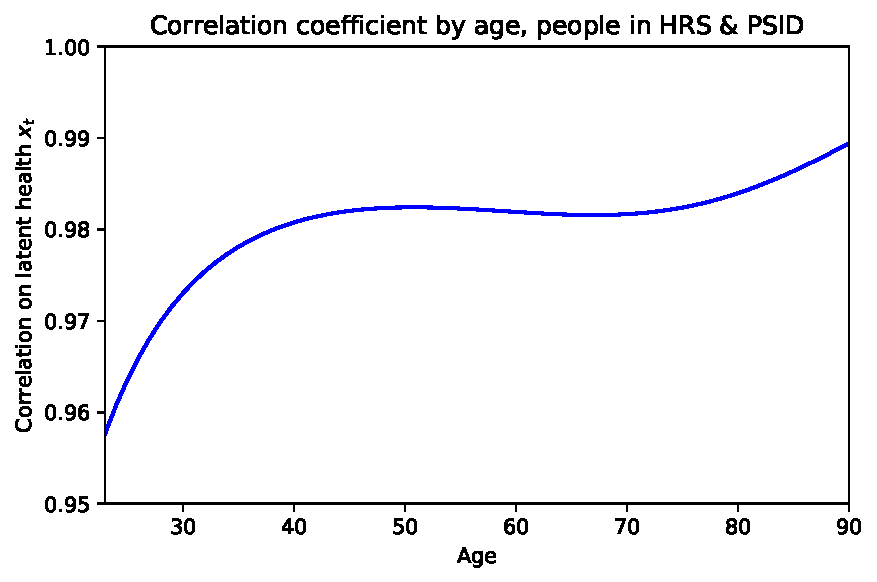
\includegraphics[width=\textwidth]{\FigsDir/TwoStudyOver23AllCorr.pdf}
		\caption{Latent health correlation factor.}\label{fig:Correlation}
	\end{subfigure}
	~
	\begin{subfigure}[b]{0.48\textwidth}
		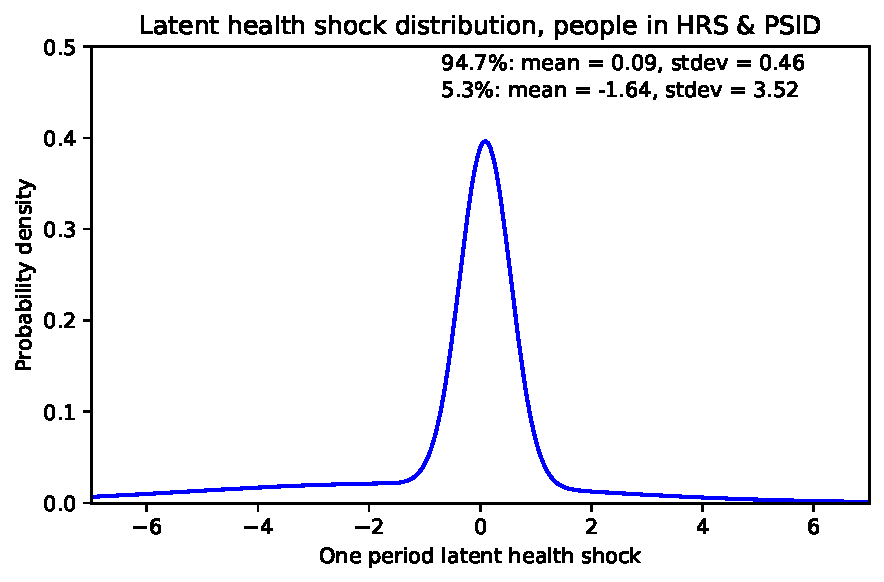
\includegraphics[width=\textwidth]{\FigsDir/TwoStudyOver23AllShockPDF.pdf}
		\caption{Health shock distribution.}\label{fig:HealthShockDstn}
	\end{subfigure}
	\caption{(a) Estimated latent health correlation factor by age, annual frequency. (b) Estimated distribution of health shocks, set to be mean zero and variance one.}
\end{figure}

Figure \ref{fig:Correlation} plots the estimated correlation coefficient by age for the specification with both sexes. At the estimated parameters, $\Corr_\Age$ rises from about 0.96 early in adulthood, then levels off near 0.982 around age 40, with a slight increase again in old age. The finding that latent health is highly persistent stands in contrast to the health processes typically calibrated in structural models, which rely on only one-wave-ahead SRHS transitions. However, my estimates are comparable to those from  the preferred specification of \cite{Lange12} using HRS data, or the persistence coefficients estimated by \cite{HosseiniZhao21a} using both HRS and PSID data.

Reporting error shocks are estimated to be highly heteroskedastic across individuals. About 8 to 10\% of the population is found to have a standard deviation of reporting shock about twice as large as the population average (normalized to one); the remainder are split about evenly between individuals with reporting errors of average magnitude and those with errors around half the average. That is, about 45\% of the population are judged to be four times more accurate than the least reliable 9\% of with respect to reporting their SRHS based on their true latent health.

In each specification, the difference between consecutive cut points ranges is consistently around 1.8.\footnote{Recall that $\Cut_1$ is normalized to 0 and thus not estimated.} To interpret this span in the context of heteroskedastic reporting behavior, consider an individual whose latent health is very close to the cut point between good and very good health. In the specification with both sexes, this corresponds to $\Health_{it} \approx \hat{\Cut}_3 / \hat{\LatentParam}_1 = 3.516 / 0.433 = 8.12$. An individual accurately reporting their health would say that their SRHS is good or very good ($\Report_{it}=3$ or $4$), but what is the probability that they say otherwise? Someone who is type $k_i=1$, with a large standard deviation of reporting errors ($\hat{\ReportStd}_1 = 2.025$), would say they are in excellent health with probability $\Phi(-(\hat{\Cut}_4 - \hat{\Cut}_3)/\hat{\ReportStd}_1) \approx 18\%$, and in fair or poor health with probability $\Phi((\hat{\Cut}_2 - \hat{\Cut}_3)/\hat{\ReportStd}_1) \approx 19.3\%$. In contrast, a respondent who is type $k_i = 2$, with the smallest reporting errors ($\hat{\ReportStd}_2 = 0.491$), would misreport their categorical health as poor, fair, or excellent only about 0.025\% of the time.\footnote{A type 3 individual would report excellent health about 4.2\% of the time and bad health 5\% of the time.}

For an individual whose latent health is between two cut points-- say, precisely in the middle of the ``very good'' range-- the probability of making an accurate categorical health report likewise varies drastically among reporting types. Someone with $k_i=3$, whose reporting errors have a standard deviation near the population average, would report $\Report_{it}=4$ about 61.4\% of the time. Those with large or small shocks would provide an accurate report with probabilities of 35.2\% and 94\% respectively. Thus for all but the most consistent reporters, the estimation finds that SRHS is a rather noisy measure of underlying health.

With an estimated coefficient on latent health of $\hat{\LatentParam}_1 = 0.433$, consecutive categorical cut points are about 4.16 units of latent health apart on average. Health shocks $\HealthShock_{it}$ are normalized to have a standard deviation of one, but the estimation finds that they are both skewed and long-tailed, as shown in Figure~\ref{fig:HealthShockDstn}. The estimation reveals that while survey respondents will report changes in SRHS of two or more categories between consecutive waves about 10\% of the time, the probability of their true latent health crossing an entire SRHS category span with a single period's shock (i.e.\ $|\HealthShock_{it}| > 4.16$) is about 1.25\% when moving down and 0.25\% if moving up.\footnote{The HRS and PSID data are both collected biannually, so there are two model periods between observations of SRHS; this increases the probability of latent health crossing two cut points in consecutive waves. However, the basic calculation here considers an individual who is just barely within the bounds of their current category, but the population is actually distributed over the entire range.} Overall, the model judges that most observed changes in SRHS, especially large jumps, occur through reporting error.


\subsection{Model Fit to SRHS Dynamics}\label{sec:Fit}

Most fundamentally, the estimated model is able to match the cross-sectional distribution of SRHS by age, shown separately for men and women in Figure~\ref{fig:SRHSfitTwoStudy}. It is also able to accurately match the mortality profile by age and SRHS in the most recent wave (Figure \ref{fig:MortFitByHealth}).\footnote{Because death is fairly rare among the younger population, the top three categorical health states had to be combined for the data trend to be readable.} As a validation of the dataset as a representative population, the model and data both have very tight matches to the Social Security Administration's mortality table.\footnote{See the Online Appendix for a comparison of the model and data to the SSA's mortality rate by age.}

\begin{figure}
	\centering
	\begin{subfigure}[b]{0.48\textwidth}
		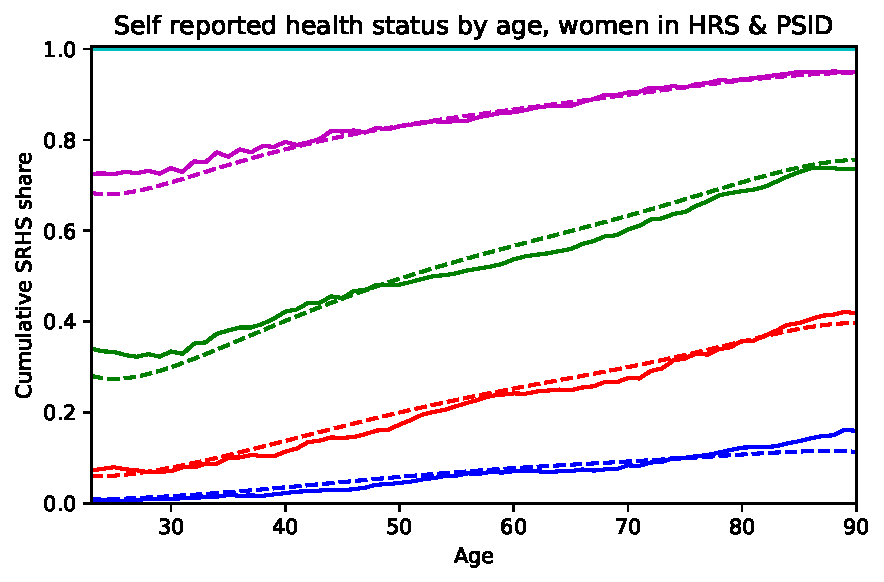
\includegraphics[width=\textwidth]{\FigsDir/TwoStudyOver23WomenSRHSbyAge.pdf}
		\caption{HRS \& PSID women}\label{fig:TwoStudyWomenSRHSfit}
	\end{subfigure}
	~
	\begin{subfigure}[b]{0.48\textwidth}
		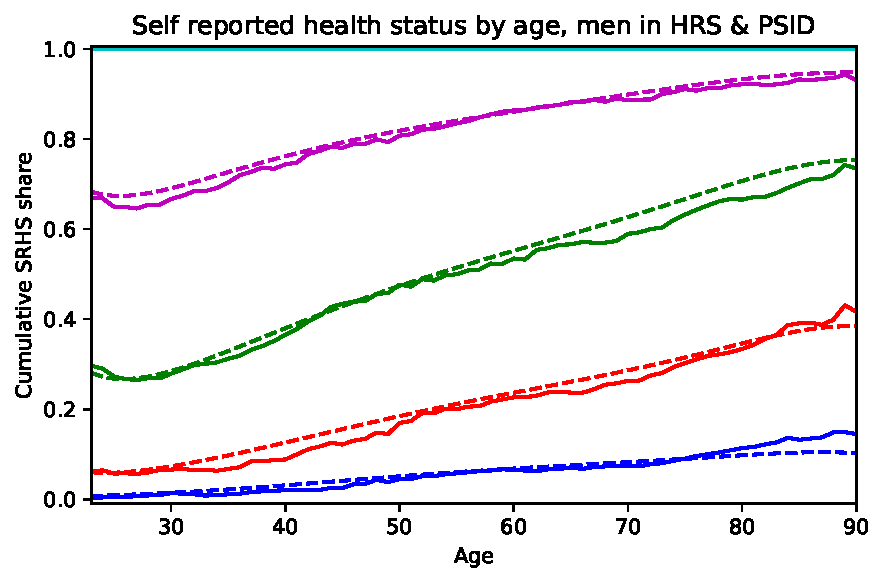
\includegraphics[width=\textwidth]{\FigsDir/TwoStudyOver23MenSRHSbyAge.pdf}
		\caption{HRS \& PSID men}\label{fig:TwoStudyMenSRHSfit}
	\end{subfigure}
	\caption{Distribution of SRHS by age, data (solid) vs estimated model (dashed).}\label{fig:SRHSfitTwoStudy}
\end{figure}

\begin{figure}
	\centering
	\begin{subfigure}[b]{0.48\textwidth}
		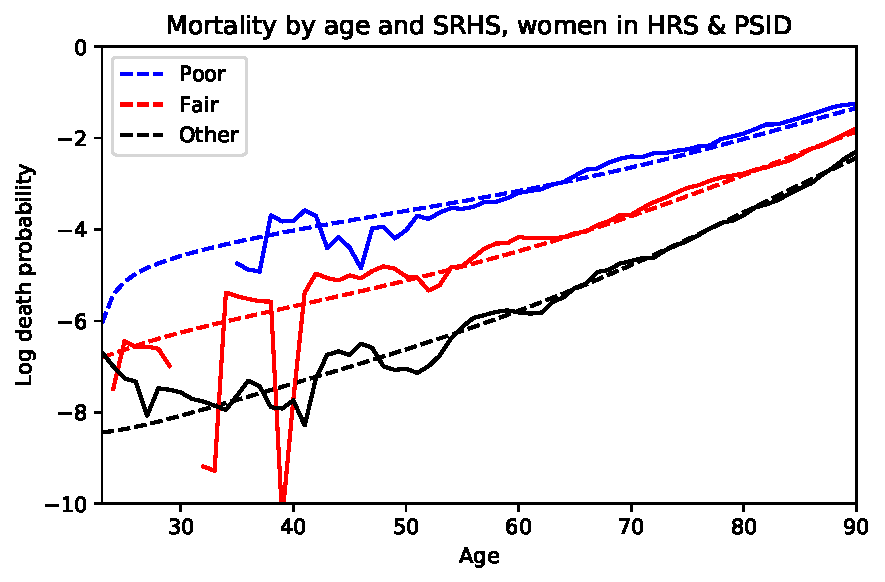
\includegraphics[width=\textwidth]{\FigsDir/TwoStudyOver23WomenMortByAgeHealth.pdf}
		\caption{HRS \& PSID women}\label{fig:TwoStudyWomenMortHealth}
	\end{subfigure}
	~
	\centering
	\begin{subfigure}[b]{0.48\textwidth}
		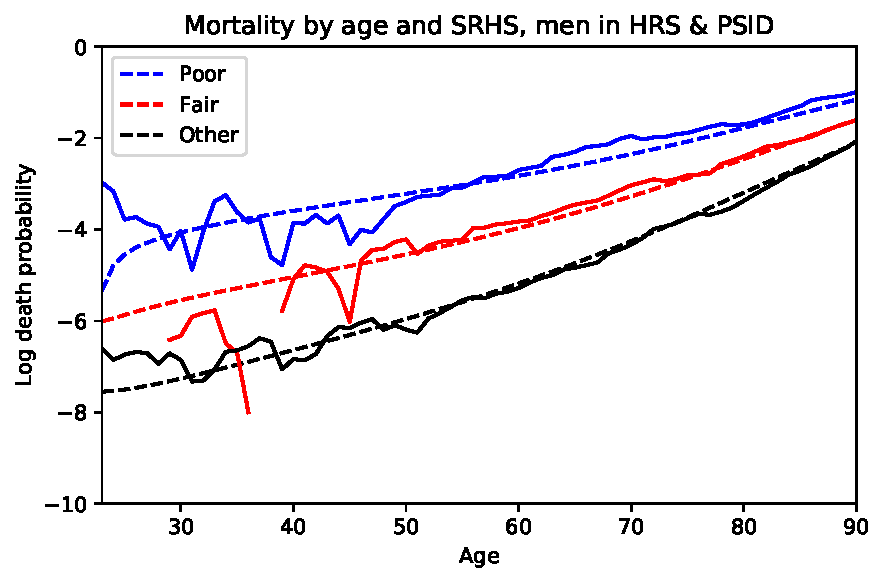
\includegraphics[width=\textwidth]{\FigsDir/TwoStudyOver23MenMortByAgeHealth.pdf}
		\caption{HRS \& PSID men}\label{fig:TwoStudyMenMortHealth}
	\end{subfigure}
	\caption{Mortality by age and health, data (solid) vs estimated model (dashed).} \label{fig:MortFitByHealth}
\end{figure}


In contrast to the ``simple dynamics'' almost universally used in structural models, the latent health model is able to match the conditional distribution of SRHS more than one period ahead.  Figure~\ref{fig:ModelTransVG} provides the estimated model analogues for Figure~\ref{fig:NaiveTransVG}. Conditional on reporting very good health in the baseline period, Figure \ref{fig:ModelTransVG} shows that the latent health model can closely match the T-waves-ahead distribution of SRHS up to twelve years in the future.\footnote{The model fit remains good up to twenty years ahead, the full length of the panel data. See the Online Appendix for comparisons of future SRHS distributions conditional on other categorical reports.} The model is least successful at predicting SRHS for older respondents (80+), undershooting the fraction who report fair health after reporting very good health at baseline.\footnote{The model is more accurate at fitting the conditional SRHS distribution for elderly who report poor, fair, or good health at baseline; see Online Appendix.} Though not shown here, the latent health model is also slightly inaccurate in projecting the future SRHS of respondents who report poor health under age 40. In both cases, there are few such observations on which to discipline the model estimates.

\begin{figure}
	\centering
	\begin{subfigure}[b]{0.45\textwidth}
		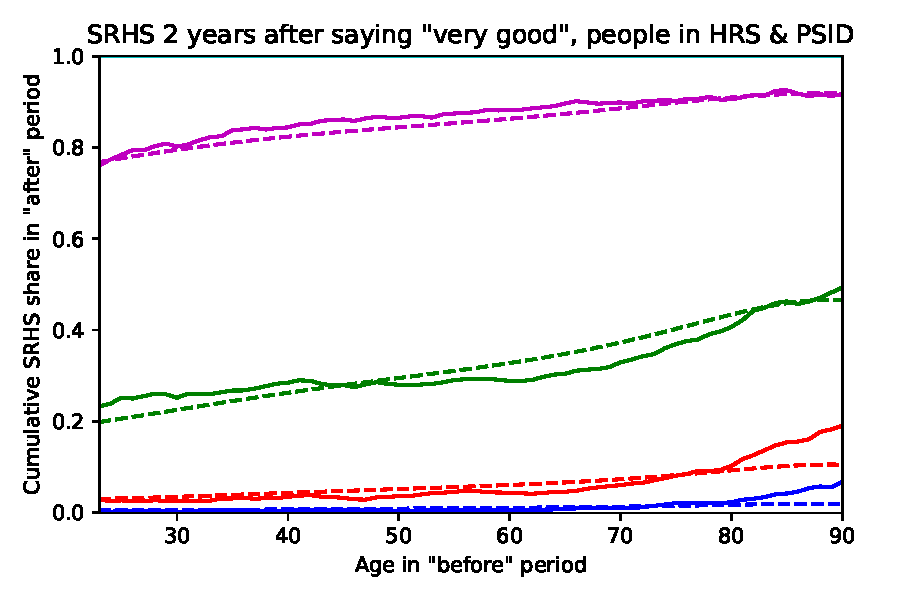
\includegraphics[width=\textwidth]{\FigsDir/TwoStudyOver23AllTransH4T2modelNoLeg.pdf}
		\caption{One wave ahead}\label{fig:Model1AheadVeryGood}
	\end{subfigure}
	~
	\begin{subfigure}[b]{0.45\textwidth}
		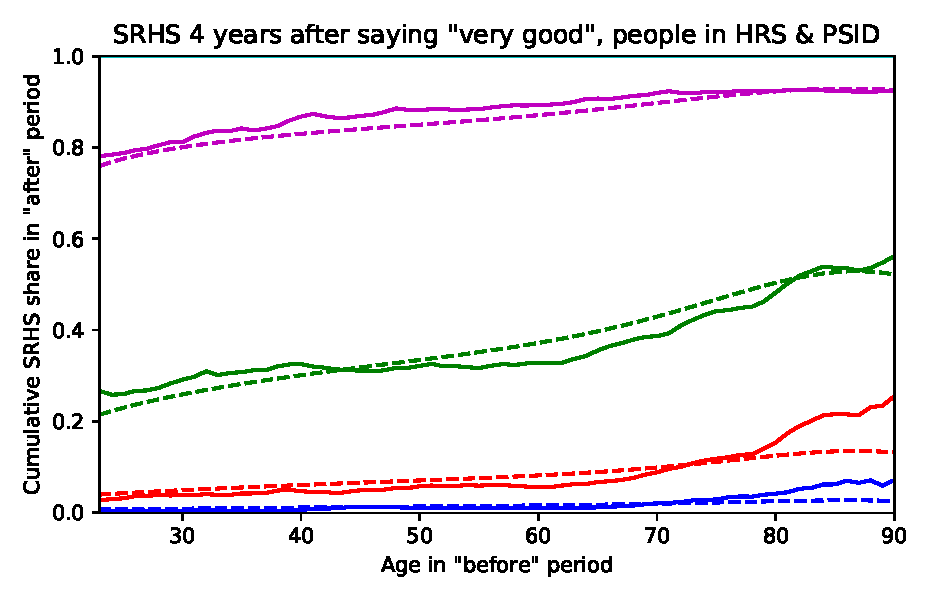
\includegraphics[width=\textwidth]{\FigsDir/TwoStudyOver23AllTransH4T4modelNoLeg.pdf}
		\caption{Two waves ahead}\label{fig:Model2AheadVeryGood}
	\end{subfigure}
	
	\begin{subfigure}[b]{0.45\textwidth}
		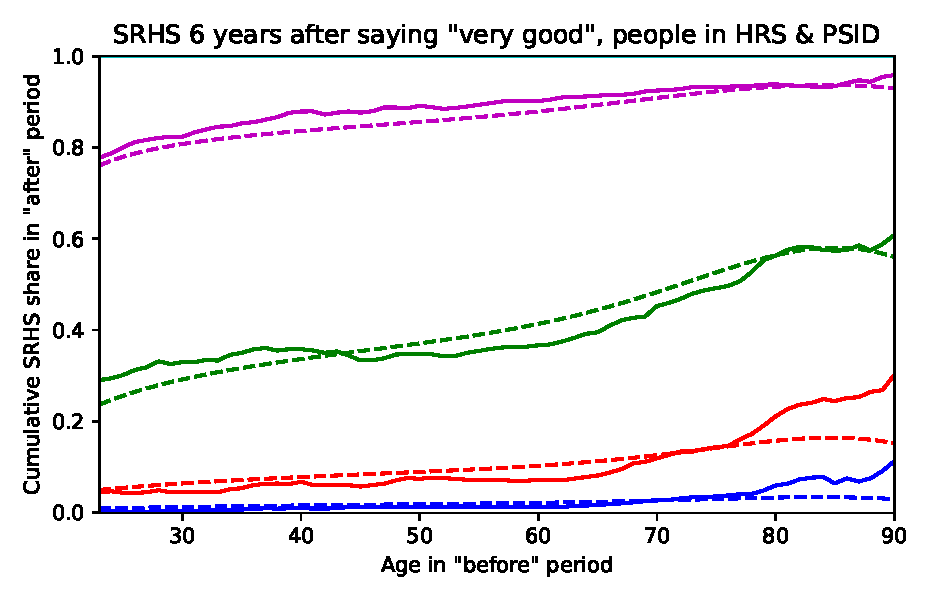
\includegraphics[width=\textwidth]{\FigsDir/TwoStudyOver23AllTransH4T6modelNoLeg.pdf}
		\caption{Three waves ahead}\label{fig:Model3AheadVeryGood}
	\end{subfigure}
	~
	\begin{subfigure}[b]{0.45\textwidth}
		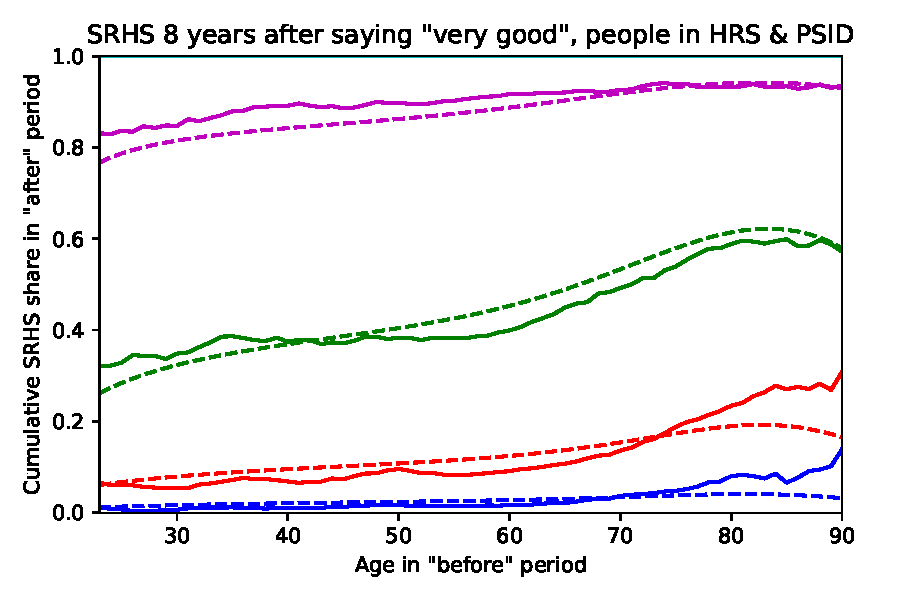
\includegraphics[width=\textwidth]{\FigsDir/TwoStudyOver23AllTransH4T8modelNoLeg.pdf}
		\caption{Four waves ahead}\label{fig:Model4AheadVeryGood}
	\end{subfigure}
	
	\begin{subfigure}[b]{0.45\textwidth}
		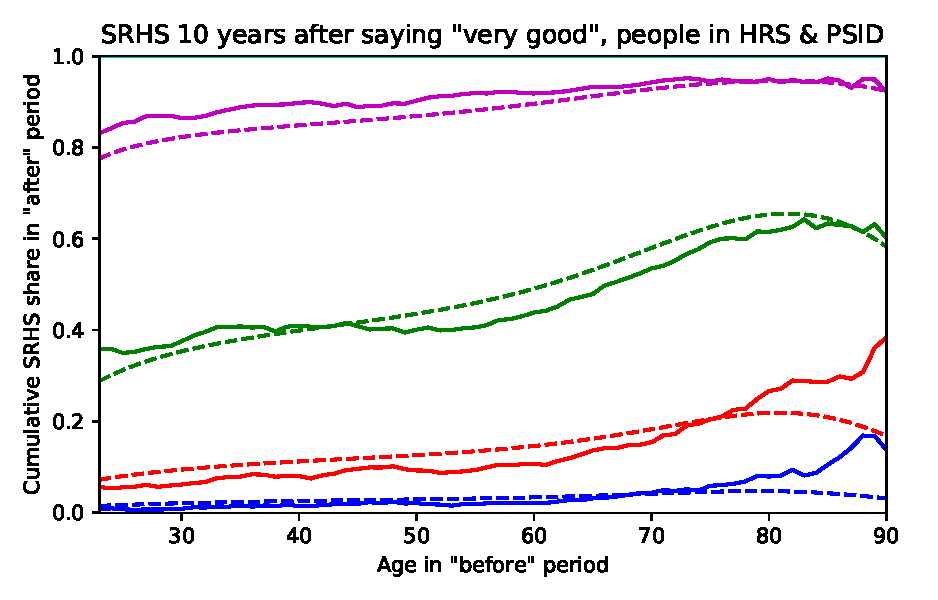
\includegraphics[width=\textwidth]{\FigsDir/TwoStudyOver23AllTransH4T10modelNoLeg.pdf}
		\caption{Five waves ahead}\label{fig:Model5AheadVeryGood}
	\end{subfigure}
	~
	\begin{subfigure}[b]{0.45\textwidth}
		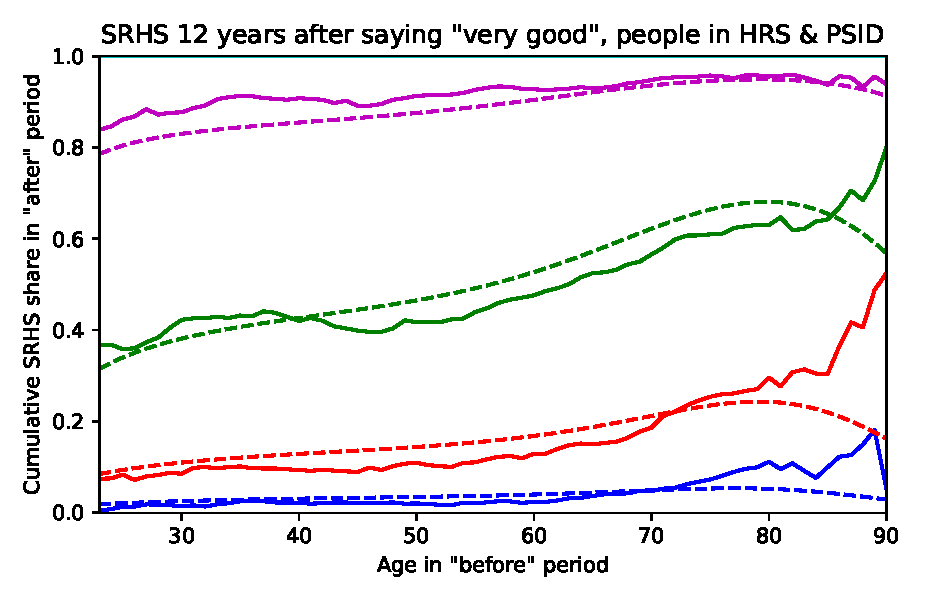
\includegraphics[width=\textwidth]{\FigsDir/TwoStudyOver23AllTransH4T12modelNoLeg.pdf}
		\caption{Six waves ahead}\label{fig:Model6AheadVeryGood}
	\end{subfigure}
	\caption{Cumulative distribution of SRHS by age conditional on reporting ``very good'' health in the baseline period in the PSID \& HRS data (solid) vs estimated model (dashed). Latent health model accurately predicts conditional distribution of SRHS well into the future, in contrast to predictions from simple dynamics.}\label{fig:ModelTransVG}
\end{figure}


\cite{DeNardi18} directly incorporate duration dependence and unobserved heterogeneity into the dynamics of a binary health state in order to match the non-Markov behavior of SRHS.\footnote{Their model is estimated on a sample of PSID men, using annual data from the 1984 to 1997 waves.}  The latent health model is able to reproduce this feature of the data, as more consecutive periods in the ``healthy'' or ``unhealthy'' groups of SRHS categories indicates that the individual's latent health is far from the cut point between fair and good and thus decreasingly likely to report a transition. Moreover, respondents who are more accurate in reporting their SRHS based on their true latent health are less likely to exhibit spurious transitions into (or out of) bad health, and thus long spans in either health group are predictive of future similar reports.

\begin{figure}
	\centering
	\begin{subfigure}[b]{0.48\textwidth}
		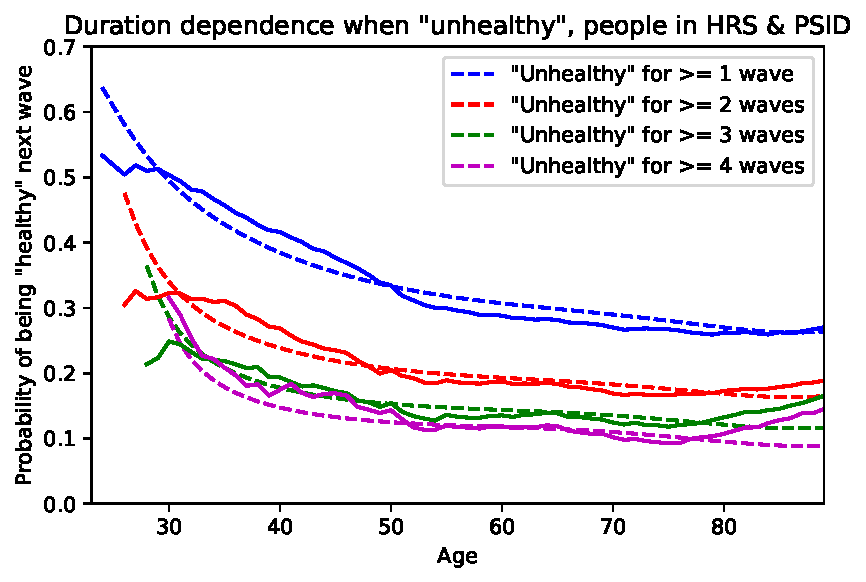
\includegraphics[width=\textwidth]{\FigsDir/TwoStudyOver23AllDurDepT4B2G.pdf}
		\caption{Duration dependence of bad health}\label{fig:DurDepTwoStudyAllB2G}
	\end{subfigure}
	~
	\begin{subfigure}[b]{0.48\textwidth}
		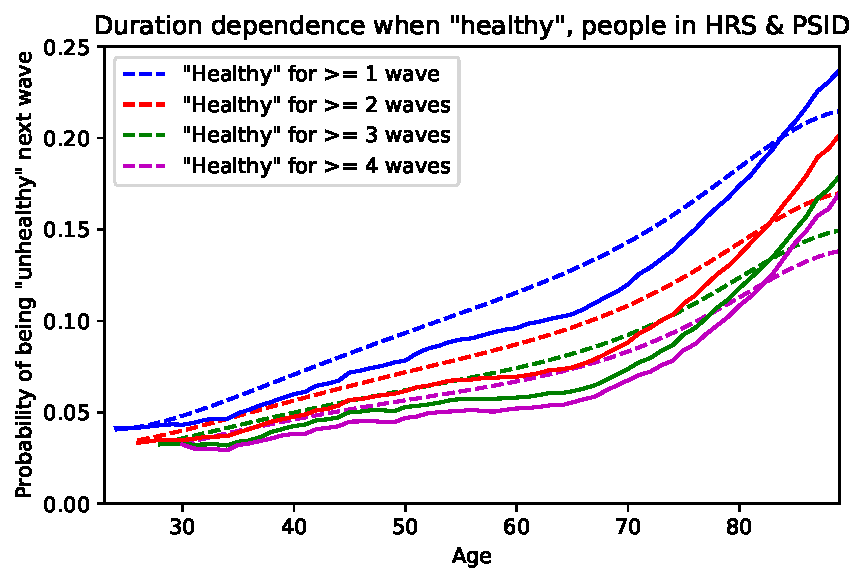
\includegraphics[width=\textwidth]{\FigsDir/TwoStudyOver23AllDurDepT4G2B.pdf}
		\caption{Duration dependence of good health}\label{fig:DurDepTwoStudyAllG2B}
	\end{subfigure}
	\caption{Duration dependence of being ``healthy'' and ``unhealthy'' as seen in survey respondents (solid) vs estimated model (dashed).  A wave represents the two years between data collection in the HRS and PSID.}\label{fig:DurDepTwoStudyAll}
\end{figure}

Using the standard definition of binary health, Figure \ref{fig:DurDepTwoStudyAllB2G} plots model and data probabilities of transitioning from being unhealthy to healthy from one wave to the next, conditional on the number of consecutive waves that a PSID or HRS respondent has reported an unhealthy SRHS; Figure \ref{fig:DurDepTwoStudyAllG2B} plots transitions from healthy to unhealthy SRHS.  Under the basic SRHS dynamics usually used in structural models, the probability of transitioning between binary health states is constant with respect to tenure in that group; graphically, the dashed model lines would be coincident, badly fitting the data. In contrast, the latent health model is able to match both the extent of duration dependence (the vertical gaps among the four data trends) and the age-trend of transition probabilities. This fit is nearly perfect for transition probabilities from unhealthy states, only barely deviating beyond age 80, and has a slight shape mismatch for transitions from healthy states.

The latent health model is also able to accurately fit the number of future waves in which an individual will report being unhealthy conditional on being unhealthy in the baseline period. Figure~\ref{fig:SRHSfreqUTwoStudy} plots the frequency of bad health over the next six waves in the HRS and PSID data versus the latent health model's prediction (conditional on survival and observation for those twelve years, in both cases).\footnote{These panels are analogous to DeNardi et al's Figure 5, which plots frequencies for men who are exactly 55 years old at baseline and in good health. For a direct comparison to their figure, see the Online Appendix.} For each age group, the latent health model's predicted frequency distribution (green) very closely matches the empirical distribution (blue). In comparison, while the simple SRHS dynamics used by most structural modelers generates a decent match to the frequency of bad health conditional on starting in good health, its predicted frequencies starting from bad health are wildly wrong (red bars on Figure~\ref{fig:SRHSfreqUTwoStudy}). In model specifications without heteroskedasticity of reporting errors, the latent health model predicts too few respondents who persistently report bad health in every wave.

\begin{figure}
	\centering
	\begin{subfigure}[b]{0.48\textwidth}
		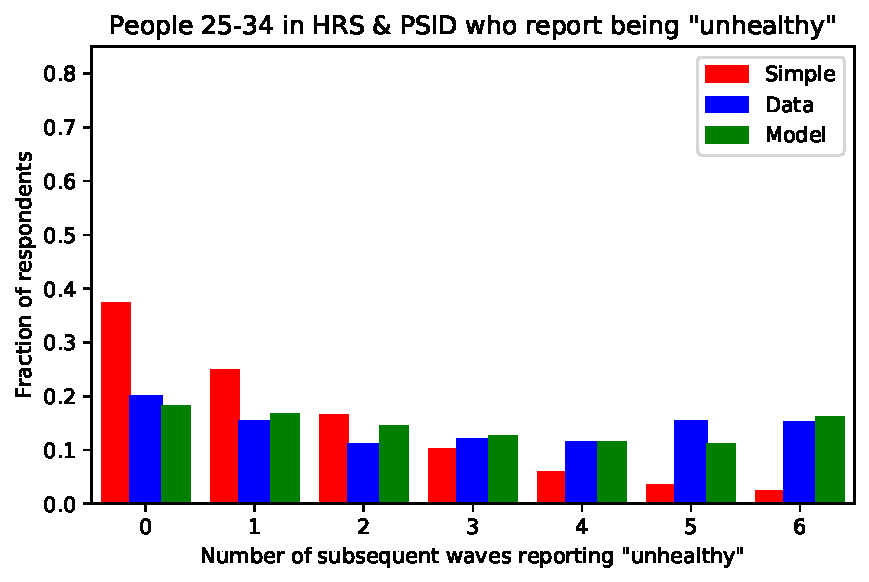
\includegraphics[width=\textwidth]{\FigsDir/TwoStudyOver23AllSRHSfreqU25to34.pdf}
		\caption{``Unhealthy'' aged 25-34 at baseline}\label{fig:SRHSfreqU25to34}
	\end{subfigure}
	~
	\begin{subfigure}[b]{0.48\textwidth}
		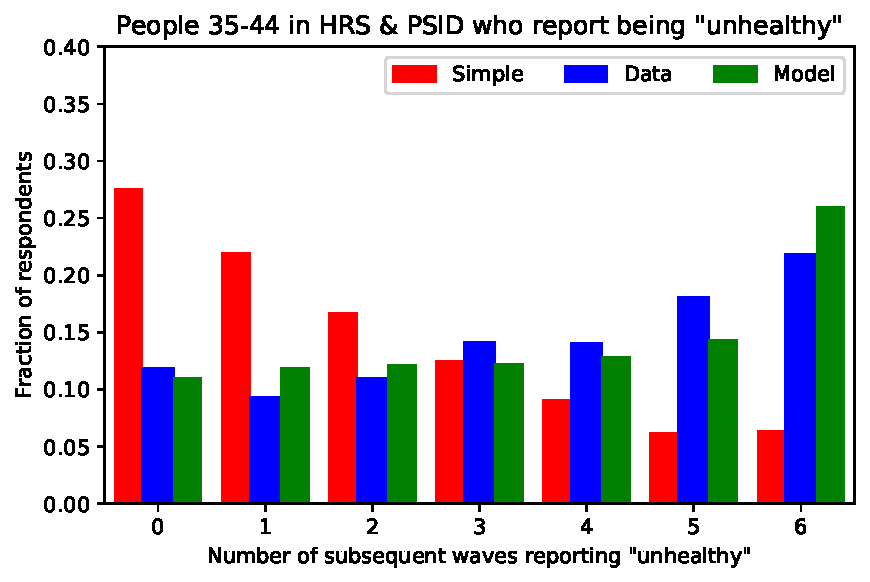
\includegraphics[width=\textwidth]{\FigsDir/TwoStudyOver23AllSRHSfreqU35to44.pdf}
		\caption{``Unhealthy'' aged 35-44 at baseline}\label{fig:SRHSfreqU35to44}
	\end{subfigure}
	
	\begin{subfigure}[b]{0.48\textwidth}
		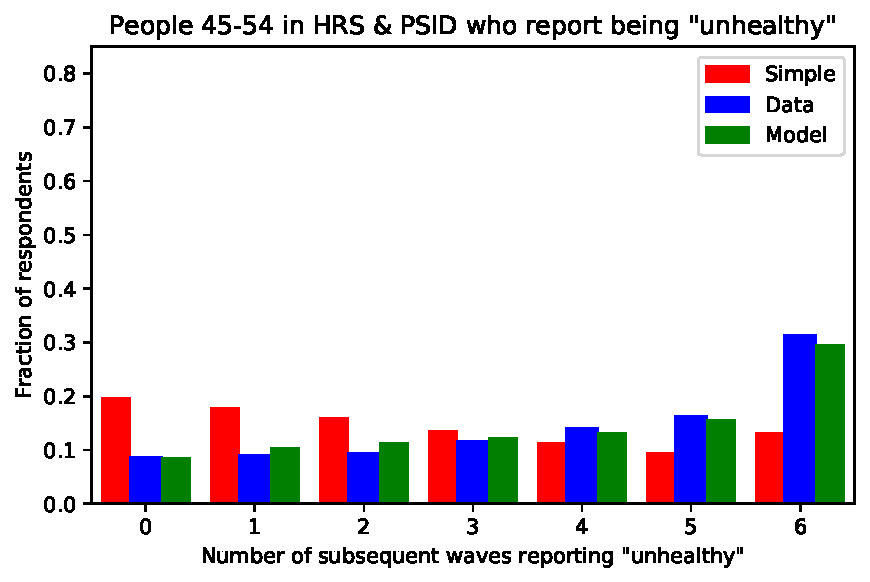
\includegraphics[width=\textwidth]{\FigsDir/TwoStudyOver23AllSRHSfreqU45to54.pdf}
		\caption{``Unhealthy'' aged 45-54 at baseline}\label{fig:SRHSfreqU45to54}
	\end{subfigure}
	~
	\begin{subfigure}[b]{0.48\textwidth}
		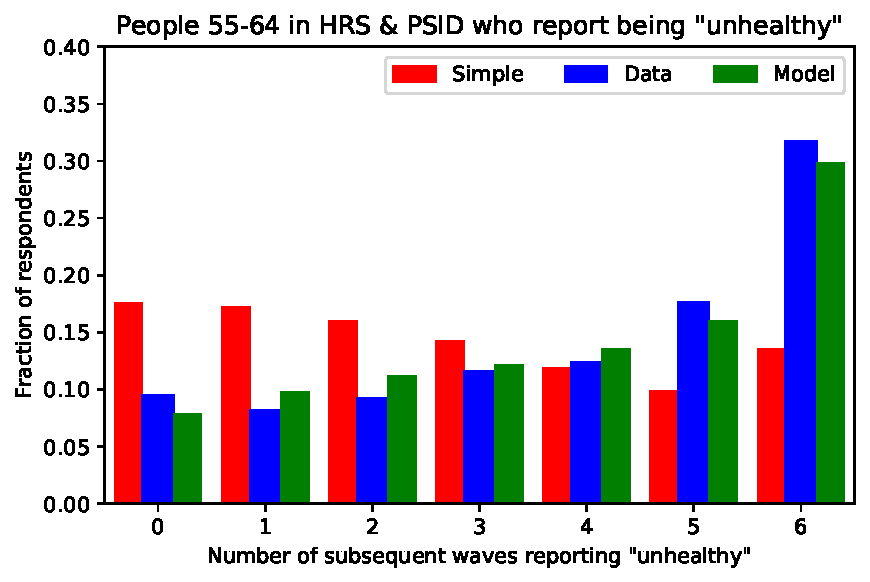
\includegraphics[width=\textwidth]{\FigsDir/TwoStudyOver23AllSRHSfreqU55to64.pdf}
		\caption{``Unhealthy'' aged 55-64 at baseline}\label{fig:SRHSfreqU55to64}
	\end{subfigure}
	
	
	\begin{subfigure}[b]{0.48\textwidth}
		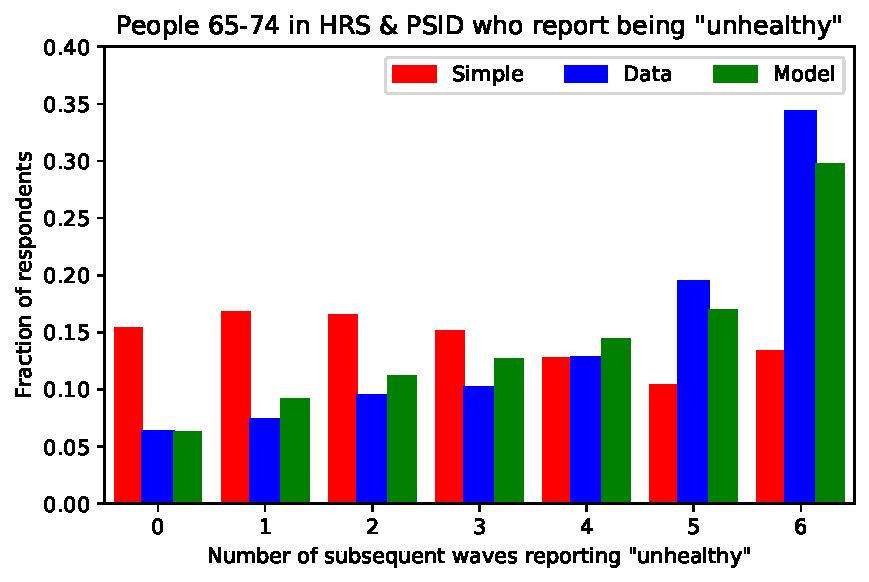
\includegraphics[width=\textwidth]{\FigsDir/TwoStudyOver23AllSRHSfreqU65to74.pdf}
		\caption{``Unhealthy'' aged 65-74 at baseline}\label{fig:SRHSfreqU65to74}
	\end{subfigure}
	~
	\begin{subfigure}[b]{0.48\textwidth}
		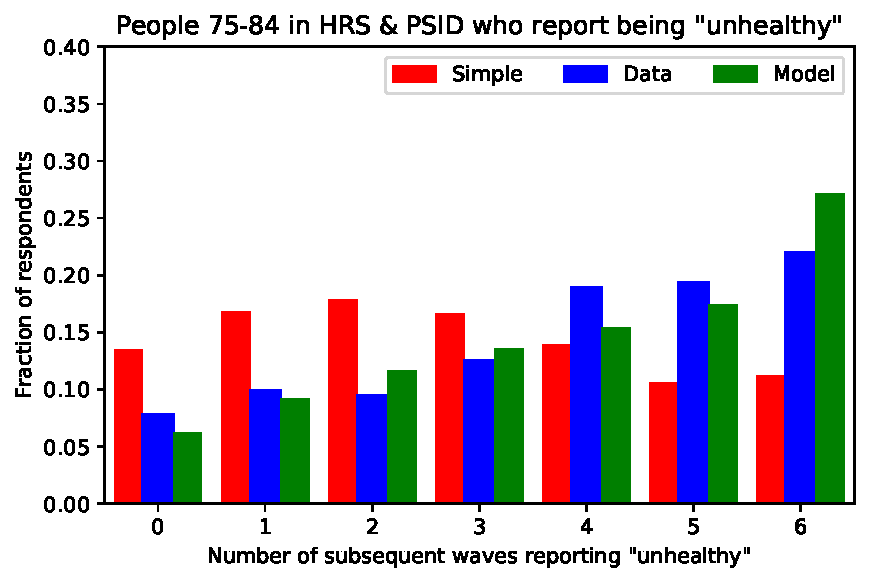
\includegraphics[width=\textwidth]{\FigsDir/TwoStudyOver23AllSRHSfreqU75to84.pdf}
		\caption{``Unhealthy'' aged 75-84 at baseline}\label{fig:SRHSfreqU75to84}
	\end{subfigure}
	\caption{Distribution of number of times reporting unhealthy SRHS by age and health over next six waves conditional on being unhealthy at baseline, data vs estimated model vs simple dynamics. Taking SRHS transition probabilities ``straight from the data'' leads to incorrect frequencies of future bad health, but latent health model fits data much better. }\label{fig:SRHSfreqUTwoStudy}
\end{figure}


\cite{Halliday11} estimates a latent health process by fitting the frequency of the three most commonly observed SRHS sequences (by age and education, with four SRHS categories); almost every single one of these sequences has the respondent reporting the \textit{same} SRHS in four consecutive waves. Figure~\ref{fig:StateCountTwoStudy} plots the distribution of the number of different SRHS categories that individuals report over seven consecutive waves of the PSID and HRS, by age group. The latent health model accurately predicts the fraction of respondents who report the exact same SRHS for twelve years (leftmost column), as well as the relative frequency of other numbers of categories visited. This stands in stark contrast to the distribution of the number of states visited generated by simple SRHS dynamics. The ``simple'' distribution significantly overshoots the proportion of respondents who report three or four categories over seven waves, and predicts very few people with the same SRHS in every period. 

\begin{figure}
	\centering
	\begin{subfigure}[b]{0.48\textwidth}
		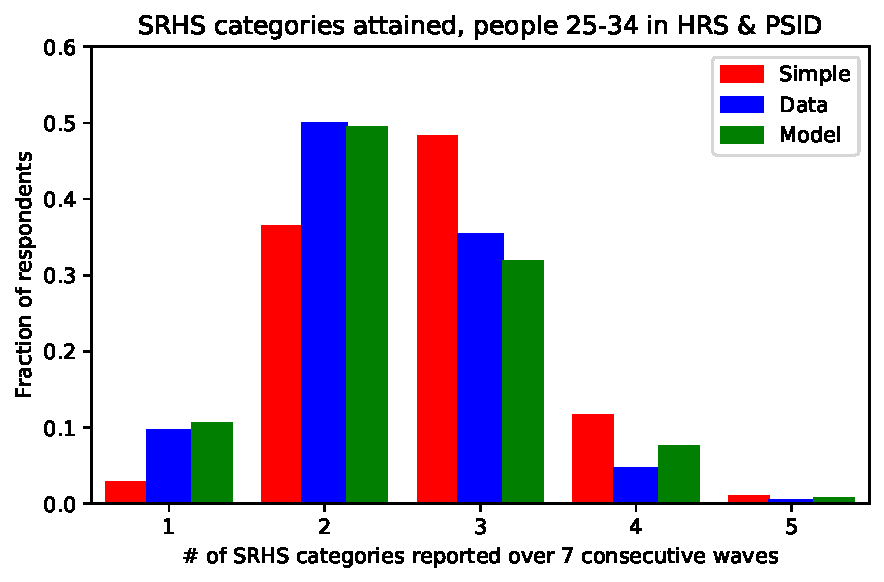
\includegraphics[width=\textwidth]{\FigsDir/TwoStudyOver23AllStateCount25to34.pdf}
		\caption{Ages 25-34 at baseline}\label{fig:StateCount25to34}
	\end{subfigure}
	~
	\begin{subfigure}[b]{0.48\textwidth}
		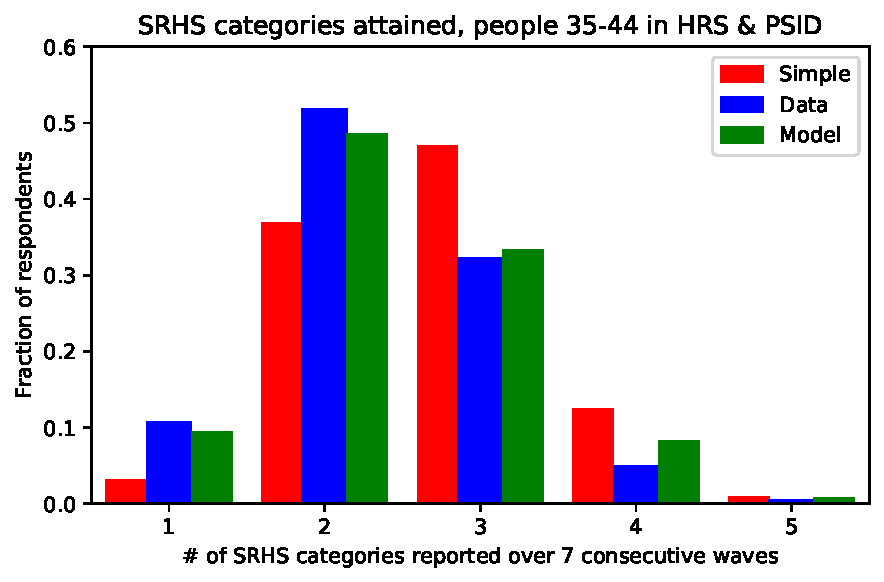
\includegraphics[width=\textwidth]{\FigsDir/TwoStudyOver23AllStateCount35to44.pdf}
		\caption{Ages 35-44 at baseline}\label{fig:StateCount35to44}
	\end{subfigure}
	
	\begin{subfigure}[b]{0.48\textwidth}
		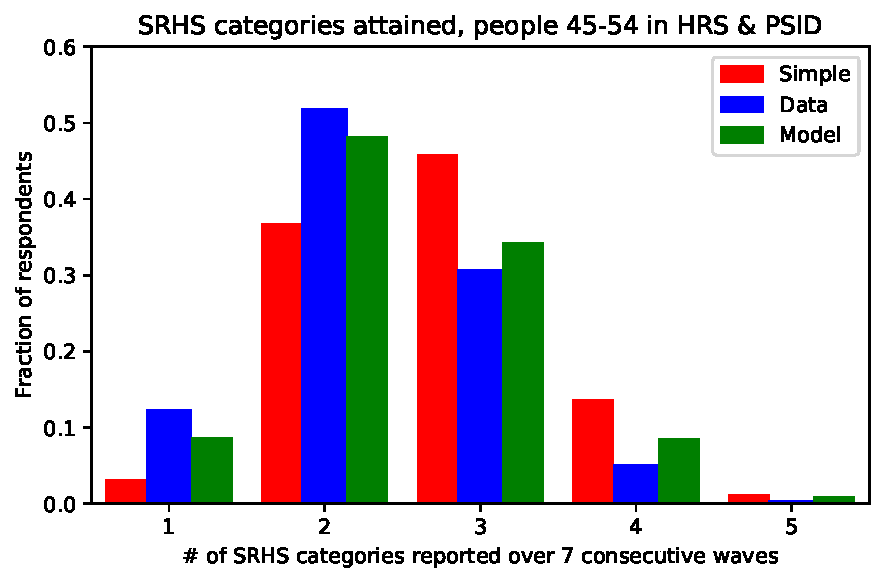
\includegraphics[width=\textwidth]{\FigsDir/TwoStudyOver23AllStateCount45to54.pdf}
		\caption{Ages 45-54 at baseline}\label{fig:StateCount45to54}
	\end{subfigure}
	~
	\begin{subfigure}[b]{0.48\textwidth}
		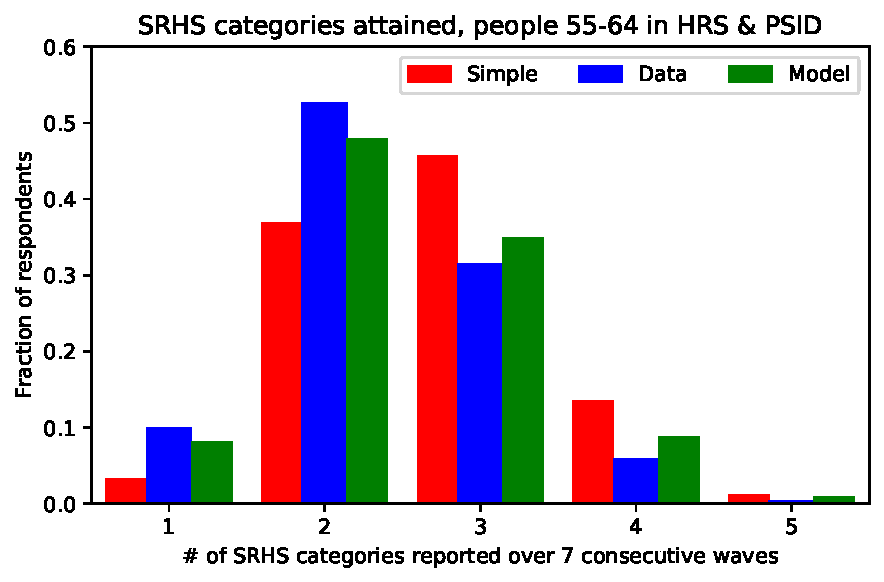
\includegraphics[width=\textwidth]{\FigsDir/TwoStudyOver23AllStateCount55to64.pdf}
		\caption{Ages 55-64 at baseline}\label{fig:StateCount55to64}
	\end{subfigure}
	
	
	\begin{subfigure}[b]{0.48\textwidth}
		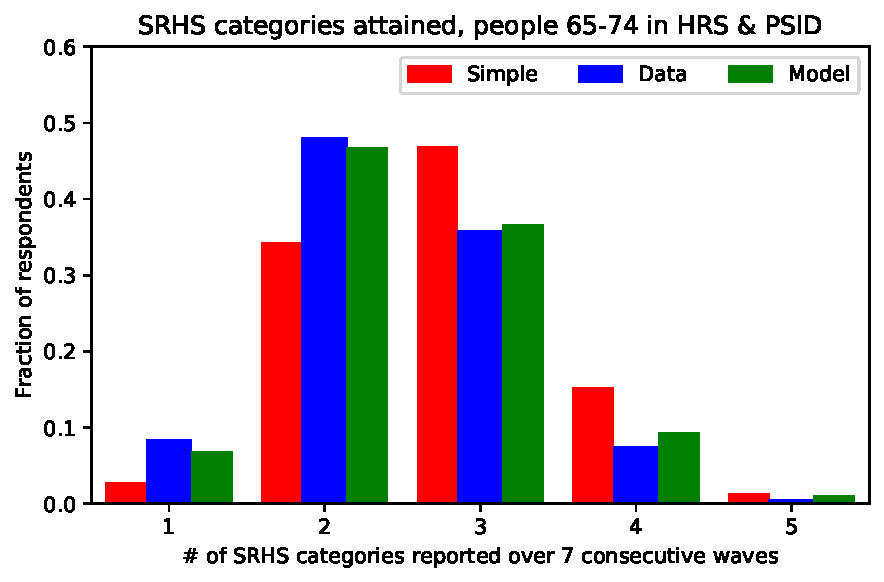
\includegraphics[width=\textwidth]{\FigsDir/TwoStudyOver23AllStateCount65to74.pdf}
		\caption{Ages 65-74 at baseline}\label{fig:StateCount65to74}
	\end{subfigure}
	~
	\begin{subfigure}[b]{0.48\textwidth}
		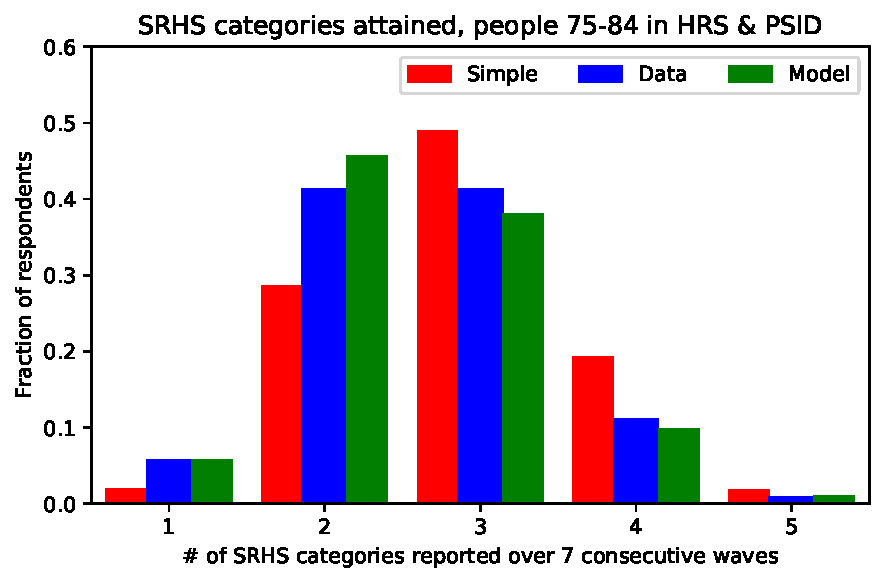
\includegraphics[width=\textwidth]{\FigsDir/TwoStudyOver23AllStateCount75to84.pdf}
		\caption{Ages 75-84 at baseline}\label{fig:StateCount75to84}
	\end{subfigure}
	\caption{Distribution of number of different health categories reported over 12 years (7 consecutive waves) using a balanced panel, model vs data vs simple dynamics. Usual assumptions about SRHS dynamics lead to agents visiting too many SRHS different categories.}\label{fig:StateCountTwoStudy}
\end{figure}




\subsection{Testing Other Model Predictions}\label{sec:Predictions}

The top-line result of \cite{Crossley02}, that 28\% of individuals will change their SRHS if asked twice in the same interview, is borne out in the Medical Expenditure Panel Survey (MEPS) data as well.  About a week after the second and fourth waves, the MEPS mails each respondent a short paper survey, the Self-Administered Questionnaire (SAQ), which includes a SRHS question nearly identically worded to the main survey. The gap of a week or two is too short a time for meaningful health shocks to occur for a significant fraction of the population, yet 38\% of MEPS respondents report a different SRHS on the SAQ than in the main survey after wave 2, and 36.5\% after wave 4.  In the context of the latent health model, responses to the two questions represent two independent draws from the reporting error distribution-- two noisy signals of the same latent health state. To test this, I calculate probability of a simulated model respondent reporting two different SRHS categories if asked twice in the same wave, finding it to be about 40-42\% at all ages (see Online Appendix for figure). This is remarkably similar to the 37\% who change their SRHS weeks apart in the MEPS, especially given that simulated agents can't even attempt to remember what they previously said.

In the health dynamics specification in \cite{DeNardi18}, transition probabilities from being healthy to unhealthy depend on once-lagged binary SRHS as well as its current value, while the probabilities of recovering from being unhealthy vary with permanent unobserved heterogeneity (with no duration dependence). However, their model assumes that the distributions of \textit{other} outcomes, such as medical expenses or death, depend only on the most recent report of SRHS. In contrast, the HRS and PSID data reveal that lagged SRHS is predictive of mortality risk. In Figure~\ref{fig:MortDurDep} I plot biannual death probability by age, decomposed by the two most recent binary SRHS reports, comparing the latent health model's predicted probabilities (dashed) to the observed rates (solid). If current SRHS were an accurate measure of true health, then the blue and red trends (currently unhealthy), as well as the green and magenta trends (currently healthy) would be coincident-- lagged SRHS would not predict mortality risk conditional on current SRHS. However, the data trends show a significant gap based on previous SRHS; the latent health model accurately predicts this differential for healthy respondents, but overshoots the information value of lagged good health (red dashed line is too low).

The latent health model also predicts other important outcomes, including labor supply on the extensive margin, at least as well as SRHS itself.\footnote{The Online Appendix shows that latent health also predicts medical spending at least as well as SRHS, using data from the MEPS (and a model specification estimated on that data) by a similar method as here.} For each pair of observations of SRHS in consecutive waves, I calculate $\widehat{\Health}_{it}$ and $\widehat{\Health^2}_{it}$ as the expectation of latent health (squared) given the econometrician's distribution after \textit{only} those two reports, conditional on the respondent's age and sex. Using a sample of HRS respondents age 50 and older, I estimate a linear probability model with the outcome as the respondent holding any job in the latter wave.  Regressing this binary outcome on $\widehat{\Health}_{it}$,  $\widehat{\Health^2}_{it}$, a dummy for holding a job in the prior wave, and a cubic of age yields an $\bar{R}^2$ of 0.608 for women ($N=88,189$ person-waves) and 0.582 for men ($N=63,548$). As a horserace comparison, a specification with a set of interacted dummies for SRHS in the latter and prior waves (i.e.\ $5 \times 5 = 25$ different constant terms) \textit{and} age dummies generates an $\bar{R}^2$ of 0.610 and 0.585 respectively.  That is, the latent health model can predict a basic measure of retirement almost exactly as well as a fully non-parametric, unrestricted model based on SRHS alone.\footnote{As further evidence that SRHS is not a perfectly accurate representation of true health, versions of this regression with dummies for current and previous SRHS (rather than their full interaction) show that SRHS two years prior is predictive of retirement, but more strongly for women than men.}

\begin{figure}
	\centering
	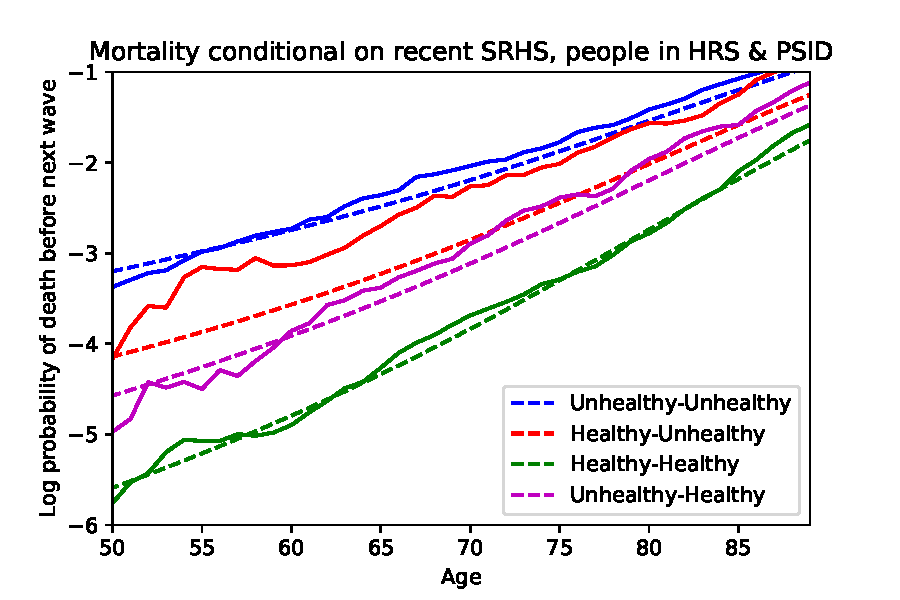
\includegraphics[scale=0.7]{\FigsDir/TwoStudyOver23AllMortDurDep.pdf}
	\caption{Dependence of mortality probability on previous and current SRHS in PSID and HRS data (solid) versus latent health model (dashed). Under health specifications used by dynamic modelers, mortality risk depends only on current SRHS.}\label{fig:MortDurDep}
\end{figure}

By assumption, the model explains short-run volatility in SRHS as reporting error around the true latent health level, and posits that individuals are heterogeneous in the magnitude of their errors. Volatility in SRHS could alternatively be explained by individuals truthfully reporting transitory shocks to their true health. These competing hypotheses can be tested by comparing how SRHS relates to \textit{objective} health measures: if the apparent heteroskedasticity in reporting errors is actually driven by heterogeneity in the extent of transitory health shocks, then SRHS should be an equally reliable measure of objective health outcomes across reporting types. The latent health model does not partition respondents by reporting type, but it does generate an \textit{ex-post} distribution of types for each respondent: $\TypeProbPcvd$ after all observations of the individual are incorporated. I calculate a version of the frailty index presented in \cite{HosseiniZhao21a} for each HRS respondent-wave used in the main estimation. These values reside on the unit interval and are meant to represent a unitary continuous measure of health.\footnote{Questions about cognition appear only in the 2002-2014 waves of the HRS, and height data was not present for all respondents. My frailty measure uses 29 binary indicators listed in Table 24 of \cite{HosseiniZhao21a} and does not include BMI or cognition measures.}

\begin{table}
\footnotesize
\singlespace
\begin{center}
\caption{Ordered Probit Regressions: SRHS on Frailty Index by Reporting Type}\label{tab:TypeProbRegressions}
\newsavebox{\TypeProbTableBox}
\sbox{\TypeProbTableBox}{  
\begin{tabular}{cccccccc}
\hline \hline
 &         & Weight & Weight & Weight & Only & Only & Only \\
 & All obs & by $\TypeProbPcvd_1$ & by $\TypeProbPcvd_2$ & by $\TypeProbPcvd_3$ & $\TypeProbPcvd_1 > 0.6$ & $\TypeProbPcvd_2 > 0.6$ & $\TypeProbPcvd_3 > 0.6$ \\
\hline
\rule{0pt}{3ex}Frailty index & -9.139    & -7.206    & -10.258   & -8.801    & -5.222    & -10.470   & -7.307 \\
                             & (4.63e-2) & (4.20e-2) & (4.91e-2) & (4.56e-2) & (2.15e-1) & (9.14e-2) & (8.59e-2) \\
\rule{0pt}{3ex}Frailty squared & 6.423    & 5.111    & 7.093     & 6.177     & 3.519     & 7.103     & 5.024 \\
                             & (6.99e-2) & (6.00e-2) & (7.59e-2) & (6.86e-2) & (3.00e-1) & (1.49e-1) & (1.31e-1) \\
\rule{0pt}{3ex}Age           & 1.03e-2   & 9.93e-3   & 1.06e-2   & 9.90e-3   & 7.89e-3   & 1.08e-2   & 7.47e-3 \\
                             & (2.45e-4) & (2.27e-4) & (2.58e-4) & (2.40e-4) & (1.16e-3) & (4.72e-4) & (4.40e-4) \\
\rule{0pt}{3ex}Sex           & -0.190    & -0.103    & -0.213    & -0.197    & 1.33e-2   & -0.194    & -0.181 \\
                             & (4.92e-3) & (4.87e-3) & (4.98e-3) & (4.91e-3) & (2.53e-2) & (8.86e-3) & (9.18e-3) \\
\hline
\rule{0pt}{3ex}Cut between        & -2.575    & -1.778    & -2.973    & -2.511    & -1.377    & -3.371    & -2.495 \\
poor \& fair                      & (1.65e-2) & (1.54e-2) & (1.74e-2) & (1.62e-2) & (8.30e-2) & (3.27e-2) & (3.05e-2) \\
\rule{0pt}{3ex}Cut between        & -1.441    & -0.936    & -1.672    & -1.393    & -0.642    & -1.788    & -1.345 \\
fair \& good                      & (1.59e-2) & (1.52e-2) & (1.66e-2) & (1.57e-2) & (8.23e-2) & (3.02e-2) & (2.95e-2) \\
\rule{0pt}{3ex}Cut between        & -0.322    & -0.174    & -0.409    & -0.311    & 0.086     & -0.407    & -0.273 \\
good \& v. good                   & (1.57e-2) & (1.51e-2) & (1.63e-2) & (1.55e-2) & (8.22e-2) & (2.96e-2) & (2.91e-2) \\
\rule{0pt}{3ex}Cut between        & 0.909     & 0.623     & 1.024     & 0.850     & 0.546     & 1.242     & 0.862 \\
v.\ good \& excel.                & (1.57e-2) & (1.51e-2) & (1.63e-2) & (1.55e-2) & (8.23e-2) & (2.97e-2) & (2.92e-2) \\
\hline
\rule{0pt}{3ex}Observations       & 197,001 & 197,001 & 197,001 & 197,001 & 7,285 & 64,674 & 56,027 \\
\rule{0pt}{3ex}Log likelihood     & -243,951.5 & -276,236.5 & -226,236.1 & -248,840.4 & -10,842.4 & -68,991.1 & -72,605.9 \\
\rule{0pt}{3ex}Pseudo $R^2$       & 0.1701 & 0.1230 & 0.2002 & 0.1614 & 0.0744 & 0.2001 & 0.1161 \\
\hline \hline
\end{tabular}
} 
\usebox{\TypeProbTableBox}  
\settowidth\TableWidth{\usebox{\TypeProbTableBox}} % Calculate width of table so notes will match  
\vspace{0.0cm} \parbox{\TableWidth}{
  \begin{flushleft}
Sample consists of all HRS respondents included in the latent health model estimation. Frailty index is constructed as described in \cite{HosseiniZhao21a}, omitting cognitive measures and BMI.
  \end{flushleft}
}
\end{center}
\end{table}


I estimate several versions of an ordered probit with SRHS as the outcome variable and using frailty (squared), age, and a dummy for sex as regressors; results are presented in Table~\ref{tab:TypeProbRegressions}. The leftmost column includes all respondents, with weights as provided by the HRS. In the next three columns, I additionally weight the observations by the \textit{ex-post} probability that each respondent is reporting type 1, 2, and 3 respectively. Recall that type 1 respondents have the largest reporting errors, and note that the estimation weighted toward this type has the lowest pseudo-$R^2$ and smallest coefficients on the frailty index among the three specifications. That is, SRHS is least predictable by an objective health index are those that the latent health model judges are the least accurate in reporting their SRHS. Conversely, type 2 individuals (with the smallest reporting shocks) have the largest frailty index coefficients and the highest pseudo-$R^2$; their objective health better predicts their SRHS. The latter three columns instead cut the data, including only respondents that the latent health model believes are at least 60\% likely to be one of the types. The same pattern is seen again: type 1 respondents have the weakest relationship between objective health and their subjective report, while type 2 respondents have the strongest. In contrast, if heterogeneity in SRHS volatility were driven by true changes in health, the relationship between frailty and SRHS would be much closer across specifications.


\section{Concluding Remarks}\label{sec:Conclusion}

I have shown that the non-Markov dynamics of SRHS can be explained with a univariate latent health model, with SRHS as a noisy signal.  The model is estimated on several well known panel surveys, using a method that tracks the econometrician's non-parametric posterior distribution about each respondent's latent health over time.  The estimated model matches both short- and long-run empirical transition probabilities, offering a significantly better fit to the data than the ``simple dynamics'' commonly used in structural models. Agents who form future expectations using the estimated latent health model will base their choice of optimal behavior on a dynamic process that more accurately reflects the prospects faced by people in the real world, relative to the very coarse simple health dynamic process.

One of the primary motivators for the literature to use a coarse discrete representation of health is that handling an additional continuous state variable is computationally costly-- the well known ``curse of dimensionality''. Given that SRHS is strongly predictive of important health-related outcomes, and that differences in these outcomes across the top three health categories are small compared to the gap with the lower two,\footnote{The difference between outcome distributions in poor and fair health is also large.} the near universal use of this representation is understandable. Moreover, the typical assumption of Markov(1) dynamics of SRHS \textit{does} preserve the overall distribution of health states by age, unconditional on prior health, many waves into the future. However, with additional evidence provided here and by \cite{DeNardi18} and \cite{HosseiniZhao21a} about longer run SRHS dynamics and more detailed features of the distribution of health shocks, continuing to make the traditional assumption is no longer tenable.

Several of the papers discussed in Section~\ref{sec:StructuralSRHS} are over a decade old as of this writing. The models presented in them were cutting edge for their time, and in some cases pushed the feasible boundary given the computational constraints faced in structural estimation. Incorporating a continuous health dimension in these projects might have rendered them impossible, but ten to twenty years of technological advancement have changed that. The field might benefit from revisiting now-classic works like \cite{RustPhelan97} and \cite{BlauGilleskie08} by extending them with a more sophisticated health process and verify that the key conclusions are sustained.

\bibliographystyle{mnwteststyle}
\bibliography{HiddenHealth}









\end{document}